\documentclass[11pt,letterpaper]{article}

\usepackage{amsmath,amssymb}
\usepackage{graphicx}
\usepackage{booktabs}
\usepackage{enumitem}
\usepackage[margin=1in]{geometry}
\usepackage[hidelinks]{hyperref}
\usepackage{xcolor}
\usepackage{caption}
\usepackage{subcaption}

\hypersetup{
  colorlinks=true,
  linkcolor=blue!45!black,
  citecolor=blue!45!black,
  urlcolor=blue!55!black
}

\graphicspath{{figures/}}

\title{Stage setting: Hubble anisotropy from an off-center CoE\\
--- derivation, Migkas ladder, CMB toy, and GR next}
\author{Chris\\{\small hedge / cosmology notes}}
\date{2026-09-20}

\begin{document}
\maketitle

\begin{abstract}
This note stages the Newtonian Sedov--Taylor (ST) + center-of-expansion (CoE)
program for an off-center observer. Homologous expansion about a real CoE yields
an isotropic apparent Hubble law; anisotropy enters only through Gauss gravity
with radially decreasing density. Against the Migkas et~al.\ (2020) $A(\ell)$
pattern (digitized Fig.~6), first-principles ST+Gauss geometry alone reaches
$R^2\approx0.543$. A diagnostic Amp$\times\sin$ phase rotation raises
$R^2_A\approx0.746$; a multiplicative $2\ell$ residual layer tuned on $A$
reaches $R^2_A\approx0.875$. A concentric blackbody-shell toy for the CMB dipole
requires $R/D\sim203$ to match Planck's $3362\,\mu\mathrm{K}$ amplitude under
$\delta T/T=(1/4)\,\delta F/F$. Numbers below are taken from on-disk fits and
files; Amp$\times\sin$ and $2\ell$ are phenomenological. Much work remains for a
true best fit. Relativity (LTB or cousin) is required as the next chapter.
\end{abstract}

\tableofcontents
\newpage

%======================================================================
\section{Basic Hubble vector derivation}
\label{sec:hubble}

Place a real geometric center of expansion (CoE) at the origin. The observer sits
at position $\vec{D}$ with $D=\|\vec{D}\|$. A source sits at $\vec{r}$
(CoE-radius $r=\|\vec{r}\|$). The observer--source separation is
\begin{equation}
\vec{d}=\vec{r}-\vec{D},\qquad d=\|\vec{d}\|,\qquad
\hat{n}=\vec{d}/d.
\end{equation}

Assume homologous expansion about the CoE,
\begin{equation}
\vec{v}(\vec{r})=H\,\vec{r},
\label{eq:homology}
\end{equation}
with the same $H$ for every tracer (Sedov--Taylor interior working assumption).
Then the observer and source velocities in the CoE frame are
$\vec{v}_O=H\vec{D}$ and $\vec{v}_S=H\vec{r}$, so the relative velocity is
\begin{equation}
\vec{v}_{\mathrm{rel}}
=\vec{v}_S-\vec{v}_O
=H(\vec{r}-\vec{D})
=H\vec{d}.
\label{eq:vrel}
\end{equation}
The line-of-sight recession speed and apparent Hubble parameter are
\begin{equation}
v_{\mathrm{los}}=\vec{v}_{\mathrm{rel}}\cdot\hat{n}=H\,d,\qquad
H_{\mathrm{obs}}\equiv\frac{v_{\mathrm{los}}}{d}=H.
\label{eq:Hobs_iso}
\end{equation}
The CoE cancels: every off-center observer measuring relative velocities sees the
same isotropic $H$. Anisotropy is \emph{not} a kinematic consequence of being
off-center under pure homology. Something must break homology---here, gravity
from a centrally concentrated, radially decreasing density (Sec.~\ref{sec:Amodel}).

\begin{figure}[ht]
\centering
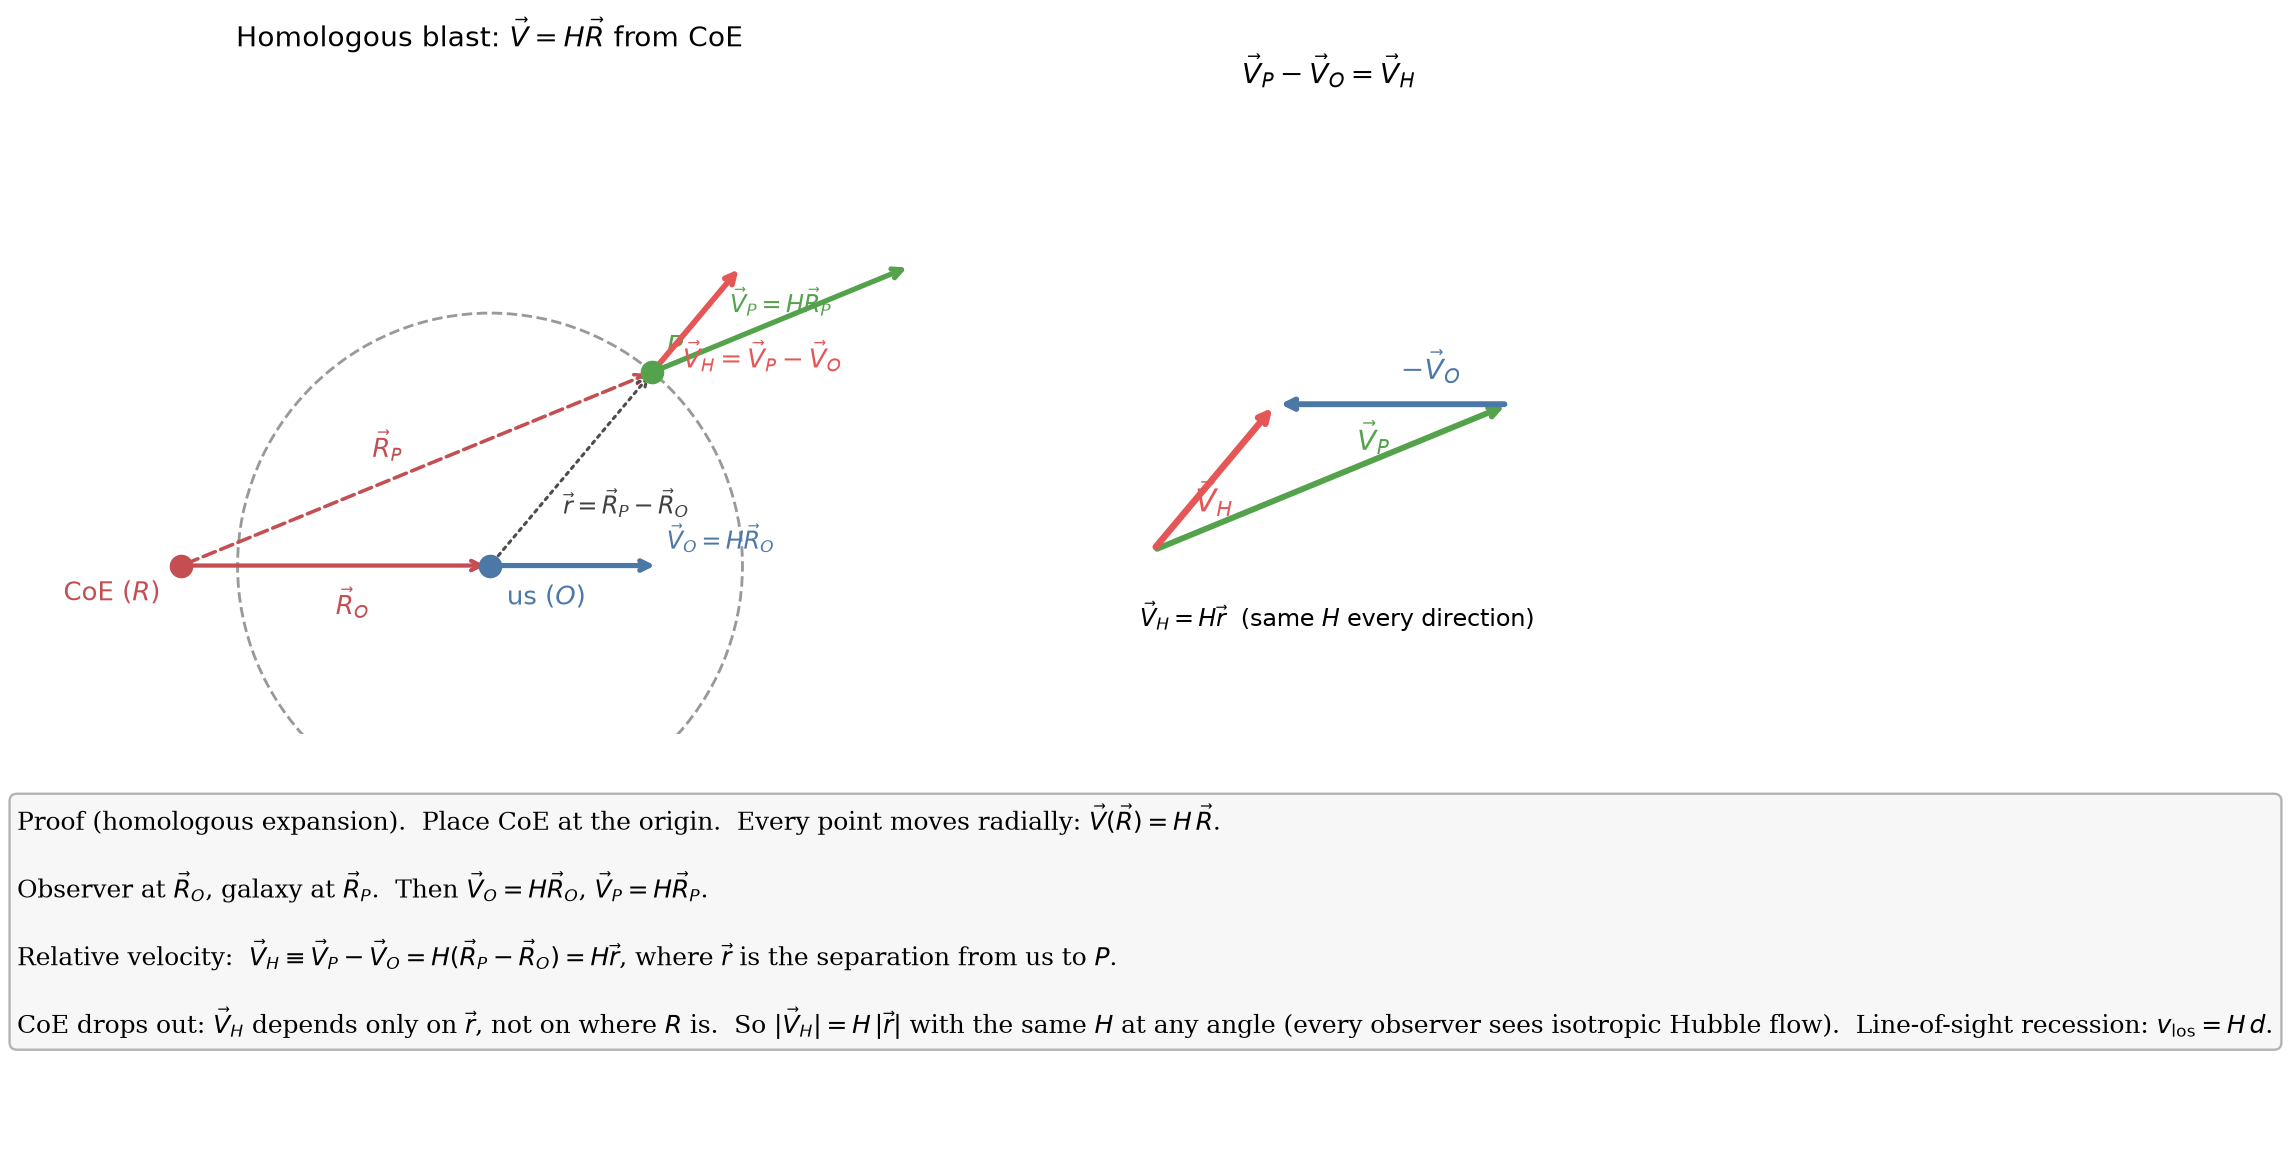
\includegraphics[width=0.88\textwidth]{hubble_from_coe_relative_velocity.png}
\caption{Homologous expansion about a CoE: absolute velocities point away from
the center, but relative velocity between observer and source is
$\vec{v}_{\mathrm{rel}}=H\vec{d}$, yielding isotropic $H_{\mathrm{obs}}=H$.}
\label{fig:hubble}
\end{figure}

%======================================================================
\section{$A$ versus angle model}
\label{sec:Amodel}

\subsection{Geometry}
Observer at distance $D$ from the CoE; sources sampled on an observer-centered
circle of depth $d$. Earth-centric angle $\varphi$ is measured from the preferred
axis $\hat{D}=\vec{D}/D$. Scale length of the mass profile is $L$; dimensionless
ratios of interest are $d/D$, $D/L$, and mass ratio $M/M_0$.

\begin{figure}[ht]
\centering
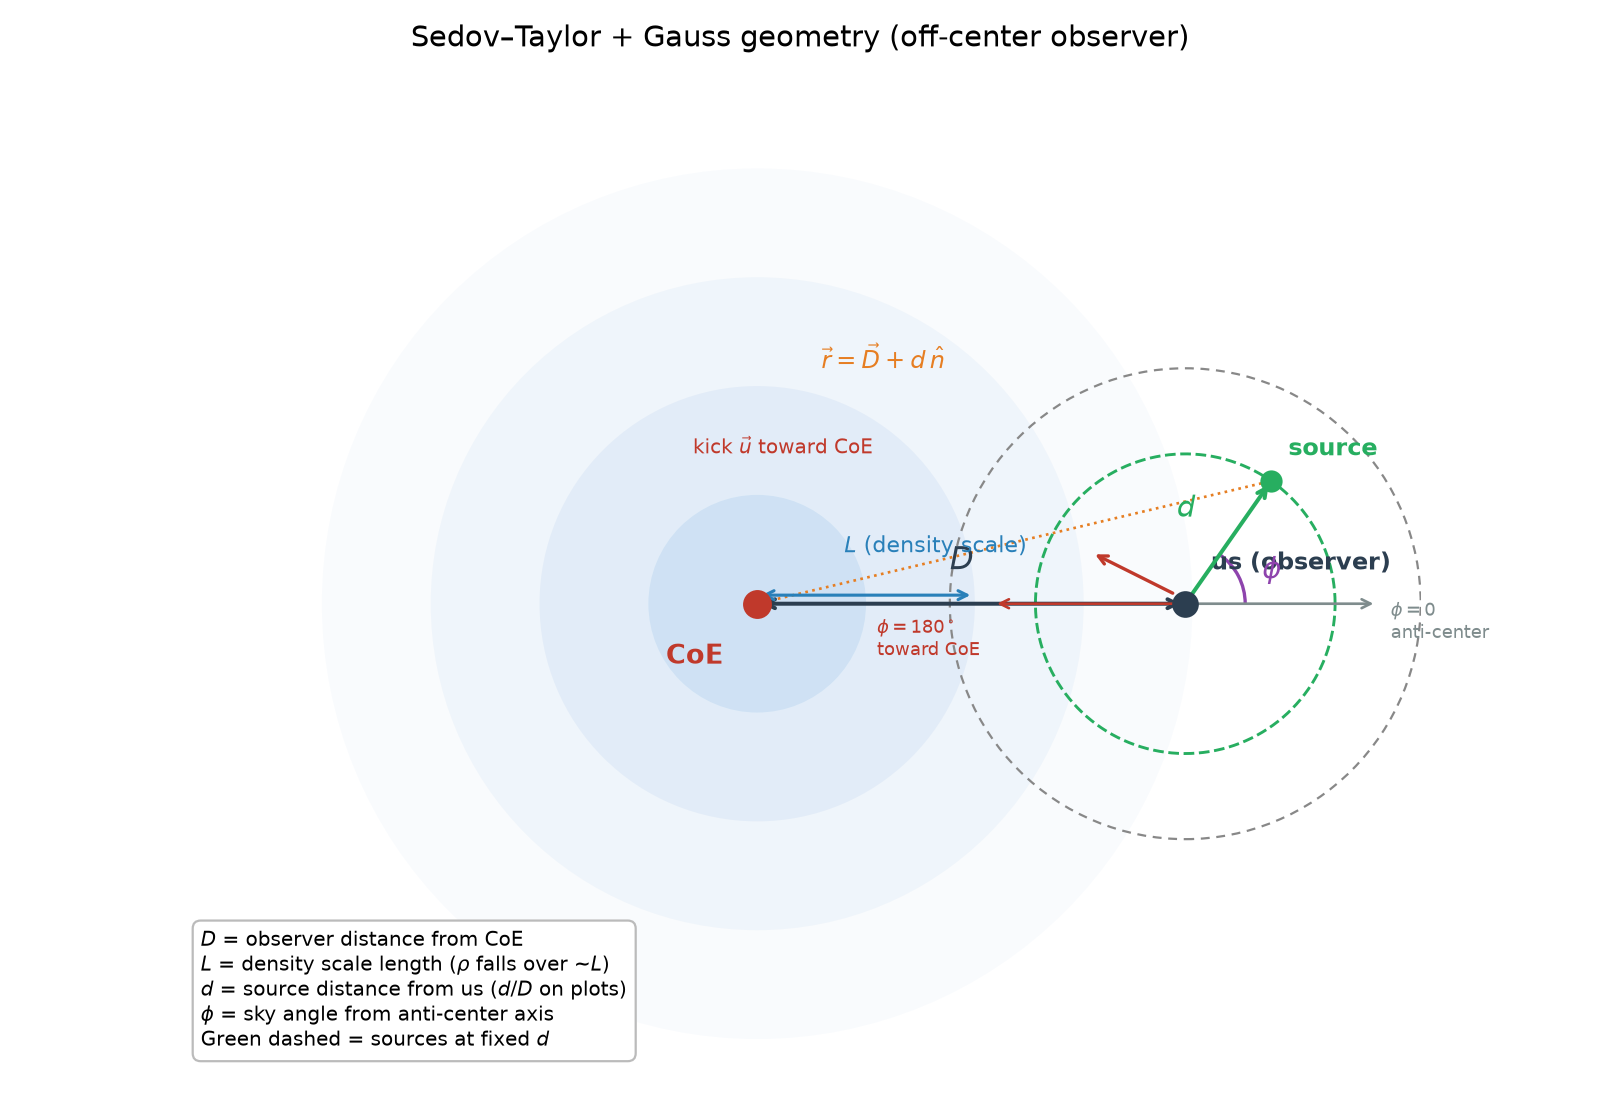
\includegraphics[width=0.72\textwidth]{geometry_CoE_observer.png}
\caption{Off-center observer geometry: CoE, observer at $D$, source distance $d$,
angle $\varphi$ from the preferred axis.}
\label{fig:geom}
\end{figure}

\subsection{ST blast + Gauss gravity with decreasing $\rho(r)$}
Classical ST blast front: $R_{\mathrm{ST}}(t)\propto t^{2/5}$,
$H=\dot{R}_{\mathrm{ST}}/R_{\mathrm{ST}}=2/(5t)$. Background velocities remain
homologous (Eq.~\ref{eq:homology}). Gravity is \emph{not} a uniform ball
($g\propto -r$). For spherical $\rho(r)$ decreasing outward, Gauss / shell
theorem gives
\begin{equation}
\vec{g}(r)=-\frac{GM(<r)}{r^2}\,\hat{r}.
\end{equation}
A dimensionless gravity strength relative to expansion is
\begin{equation}
\kappa\equiv\frac{GM(<D)}{D^3 H^2}.
\label{eq:kappa}
\end{equation}
A natural order-of-magnitude target is $\kappa\sim\Omega_m/2\approx0.15$ if one
identifies enclosed mass with a cosmic mean; fitted working values in this
program are larger (Sec.~\ref{sec:migkas}--\ref{sec:rotation}).

Peculiar velocities from gravity break homology. In the sheet AF convention used
here,
\begin{equation}
A\propto\frac{H_{\mathrm{obs}}}{H}
\end{equation}
(mean-normalized when compared to Migkas). Ideal continuous integration of gravity
along expansion history rescales amplitude ($\alpha\to\alpha_{\mathrm{eff}}$) but
does not flip the angular shape of $A(\varphi)$; expand versus collapse does.

\begin{figure}[ht]
\centering
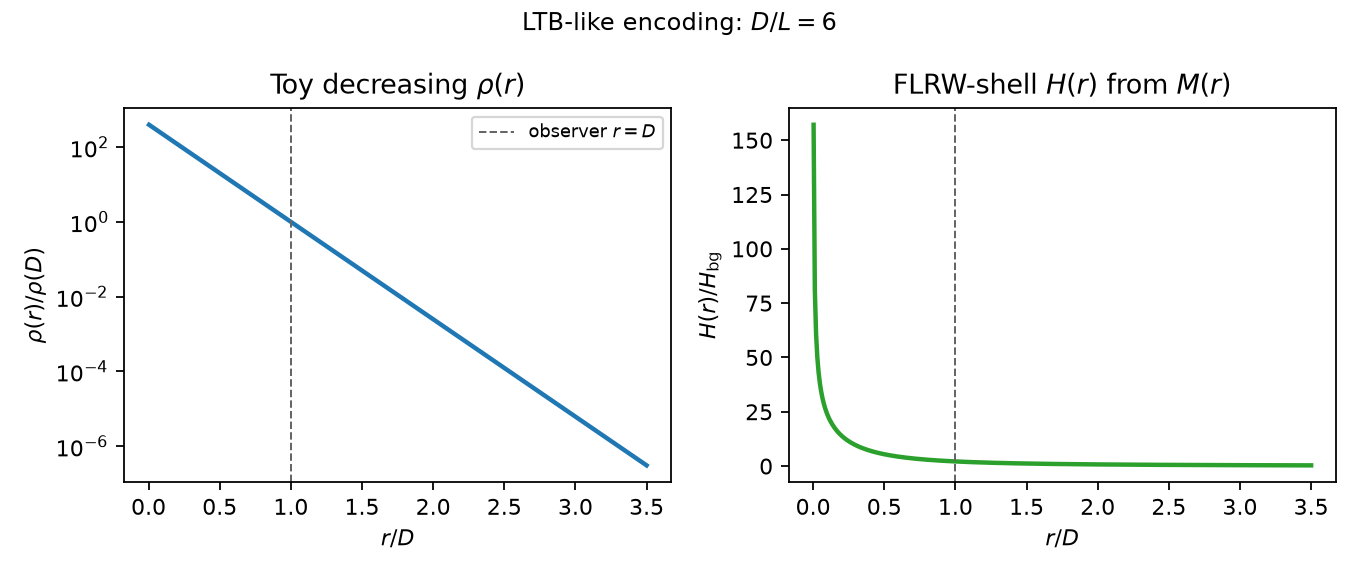
\includegraphics[width=0.78\textwidth]{toy_density_H_profile.png}
\caption{Toy density and Hubble profile versus CoE radius (from the GR Ch.~2
draft figures). Decreasing $\rho(r)$ is the ingredient that makes Gauss gravity
anisotropic for an off-center observer.}
\label{fig:rhoH}
\end{figure}

\begin{figure}[ht]
\centering
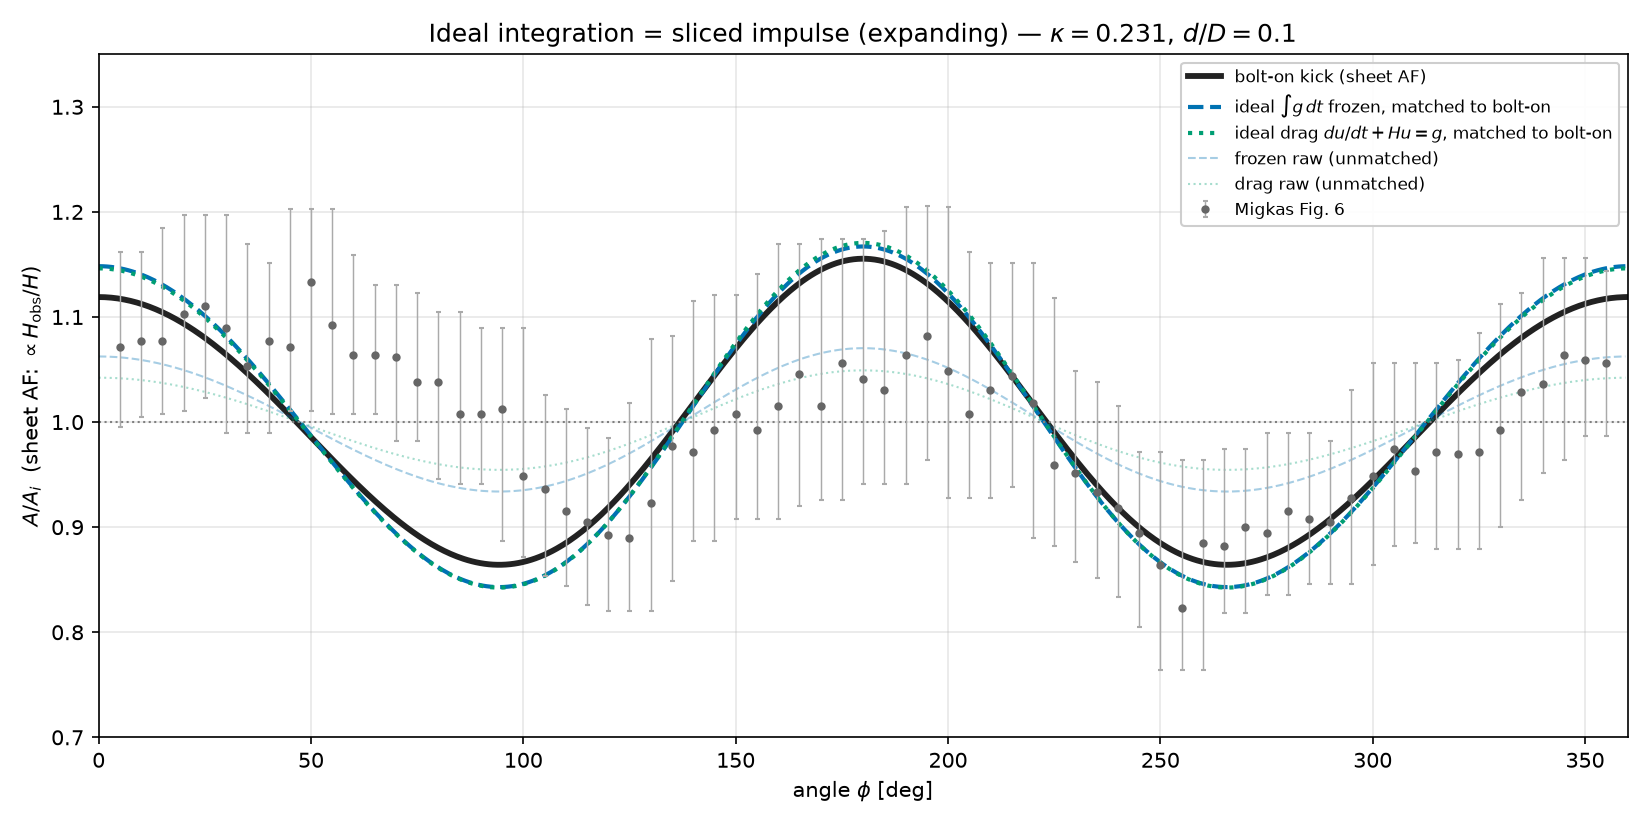
\includegraphics[width=0.88\textwidth]{A_vs_angle_ideal_integration_sheet_AF.png}
\caption{Ideal-integration ST+Gauss $A$ versus angle under sheet AF
($A\propto H_{\mathrm{obs}}/H$), compared against the Migkas longitude pattern
after axis phasing.}
\label{fig:Aideal}
\end{figure}

\paragraph{Toy-universe ranges from fits (not informal guesses).}
On-disk continuous ideal fit against digitized Migkas $A$
(\texttt{ideal\_fit\_M\_d\_D\_L\_migkas.npz}):
$d/D\approx0.76$, $D/L\approx7.62$, $\kappa\approx0.458$, $R^2\approx0.78$.
Discrete geometry-grid best (before Amp$\times\sin$ in the staged ladder):
$M/M_0=3$, $d/D=0.5$, $L\approx0.169$, $D/L\approx5.9$, $\kappa\sim0.7$,
geometry-alone $R^2\approx0.543$. These fitted ranges---not informal $3$--$4r$
guesses---are the working toy universe for this stage-setting note.

%======================================================================
\section{Observable from Migkas}
\label{sec:migkas}

Migkas et~al.\ (2020) report directional variation in the X-ray cluster
$L_X$--$T$ normalization $A$ (and related $B$) versus Galactic longitude
(their Fig.~6). Digitized points are from
\texttt{migkas/fig6\_digitized.csv} (copied into this paper's
\texttt{figures/}). Those data remain contested (calibration, absorption,
bulk flow, scatter); they are used here as the empirical angular target,
not as settled cosmology.

\begin{figure}[ht]
\centering
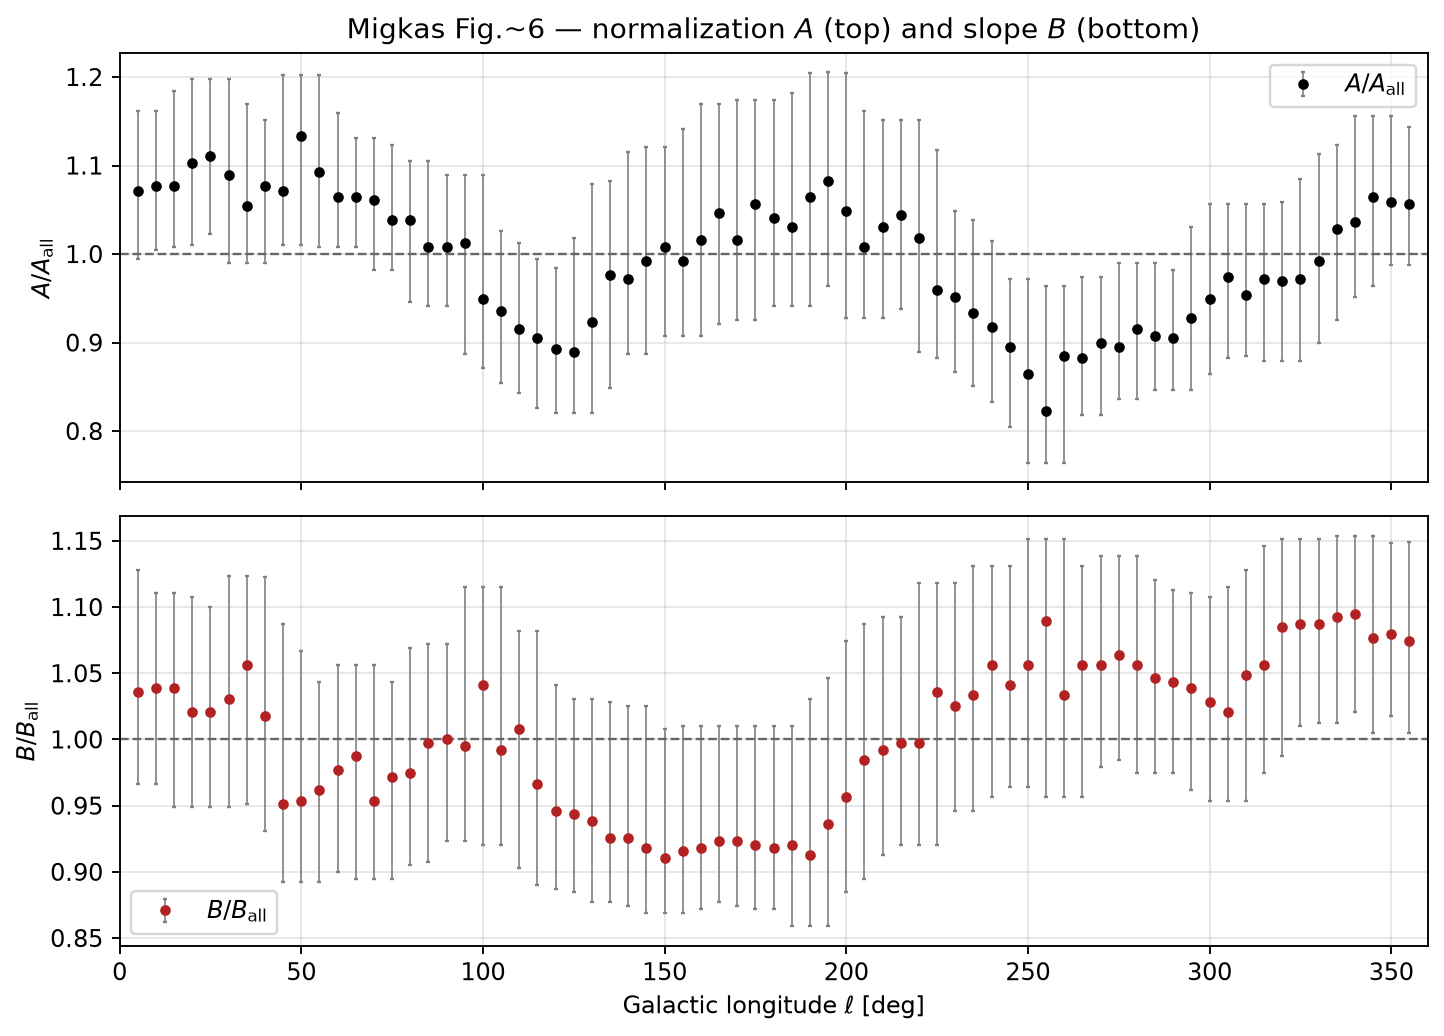
\includegraphics[width=0.92\textwidth]{AB_vs_angle_migkas_fig6.png}
\caption{Digitized Migkas et~al.\ (2020) Fig.~6: $A$ and $B$ versus Galactic
longitude, with model overlays from the ST+CoE ladder where available.}
\label{fig:migkasAB}
\end{figure}

Geometry alone (grid best cited above) gives $R^2\approx0.543$ on $A$. That is
the first-principles rung of the ladder; subsequent Amp$\times\sin$ and $2\ell$
layers are diagnostic, not derived ST+Gauss.

%======================================================================
\section{Residuals: model $A$ versus Migkas (before rotation)}
\label{sec:resid_before}

Figure~\ref{fig:resid_before} shows Migkas $A$ minus the geometry (sheet AF)
template after a least-squares affine match in amplitude/offset. Systematic
angular structure remains---the motivation for the Amp$\times\sin$ diagnostic in
Sec.~\ref{sec:rotation}.

\begin{figure}[ht]
\centering
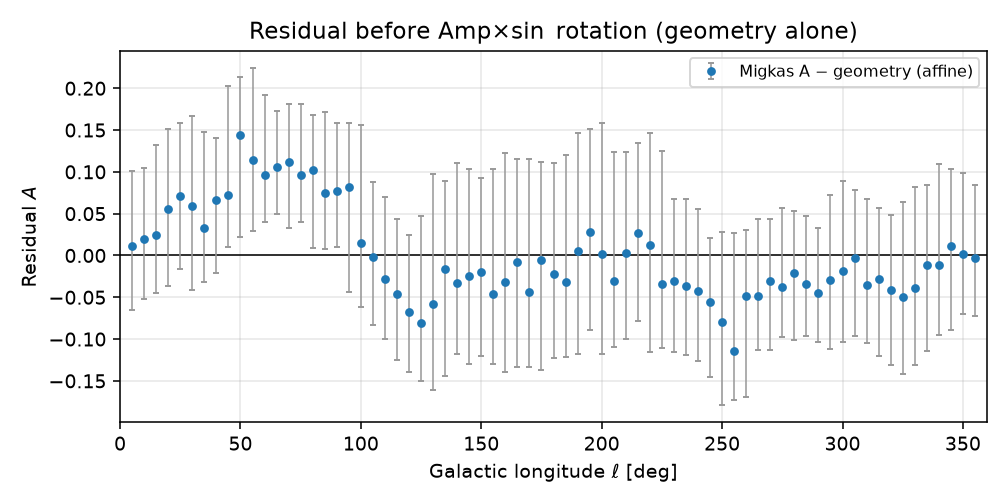
\includegraphics[width=0.92\textwidth]{residual_before_rotation.png}
\caption{Residual before Amp$\times\sin$ rotation: digitized Migkas $A$ minus
geometry (AF) template with affine match. Error bars from the digitized Fig.~6
uncertainties.}
\label{fig:resid_before}
\end{figure}

%======================================================================
\section{Rotation (Amp$\times\sin$)}
\label{sec:rotation}

A one-parameter phase alignment on the longitude circle,
\begin{equation}
A_{\mathrm{rot}}(\ell)
=
A_{\mathrm{geom}}(\ell)\,\bigl[1+\mathrm{Amp}\cdot\sin(\ell+\phi)\bigr]
\end{equation}
(with Amp and $\phi$ fitted; sheet convention), raises the $A$ match
substantially. Best Amp$\times\sin$ values used here
(from \texttt{R2\_best\_A\_B\_Amp\_phi\_summary.csv} /
\texttt{rotation\_Amp\_phi\_R2\_ranked.csv}):
\begin{equation}
\mathrm{Amp}=-0.06,\qquad
\phi\approx11.46^\circ\ (0.20\,\mathrm{rad}),\qquad
R^2_A\approx0.746.
\end{equation}
Shared opposite amplitude $\mathrm{Amp}_B=-\mathrm{Amp}_A$ gives
$R^2_B\approx0.79$ at the same $\phi$. Geometry alone was $R^2_A\approx0.543$;
Amp$\times\sin$ is a diagnostic phase knob, not a first-principles ST prediction.

\begin{figure}[ht]
\centering
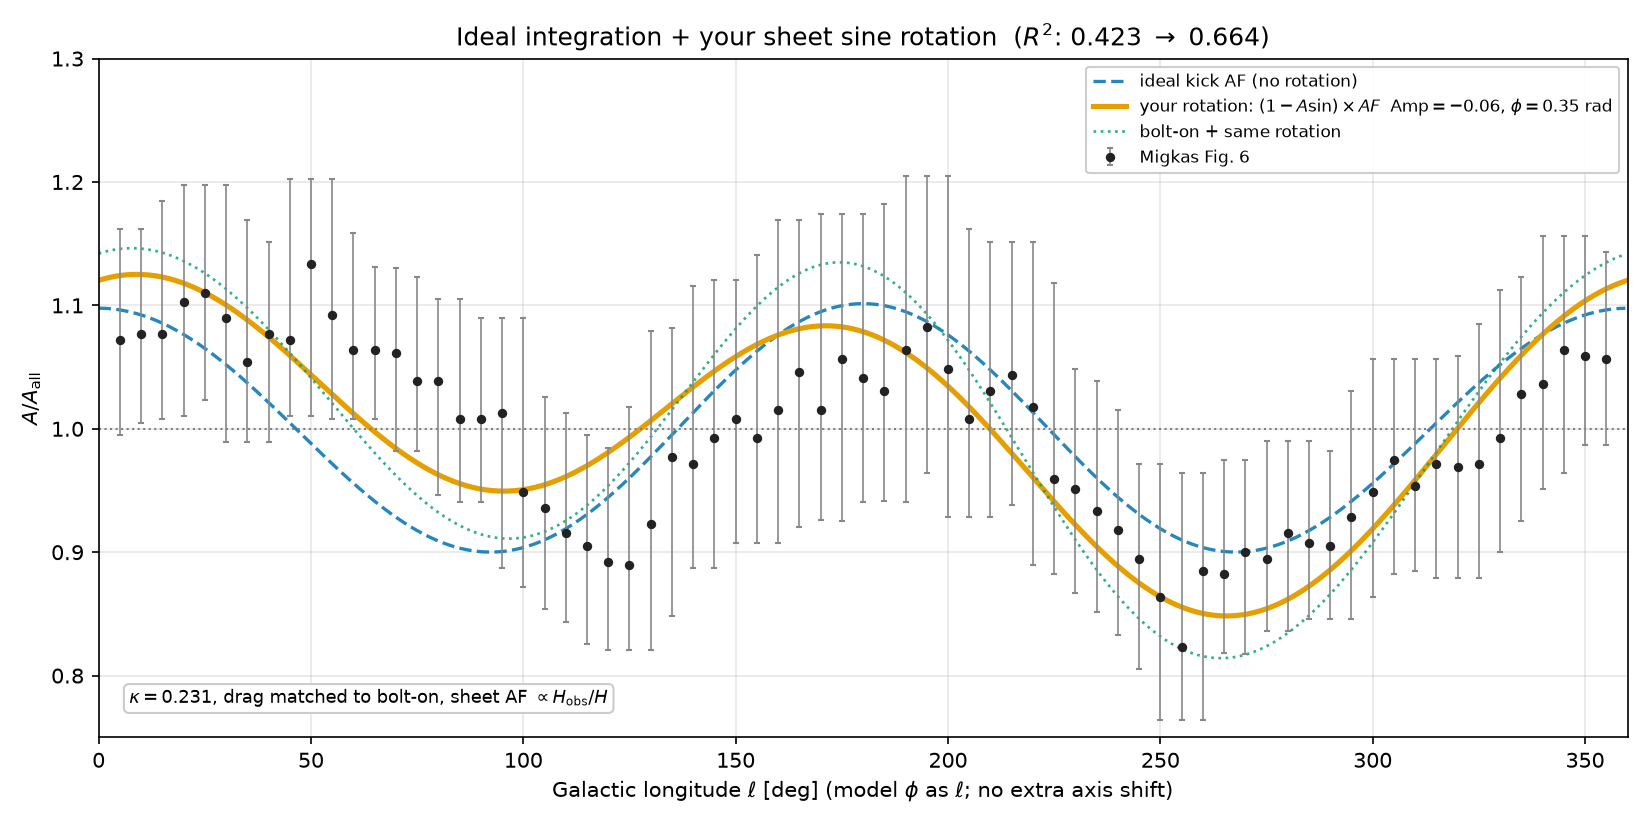
\includegraphics[width=0.88\textwidth]{A_vs_angle_ideal_plus_chris_rotation.png}
\caption{Ideal geometry $A(\ell)$ plus Amp$\times\sin$ rotation versus Migkas
points.}
\label{fig:Arot}
\end{figure}

\begin{figure}[ht]
\centering
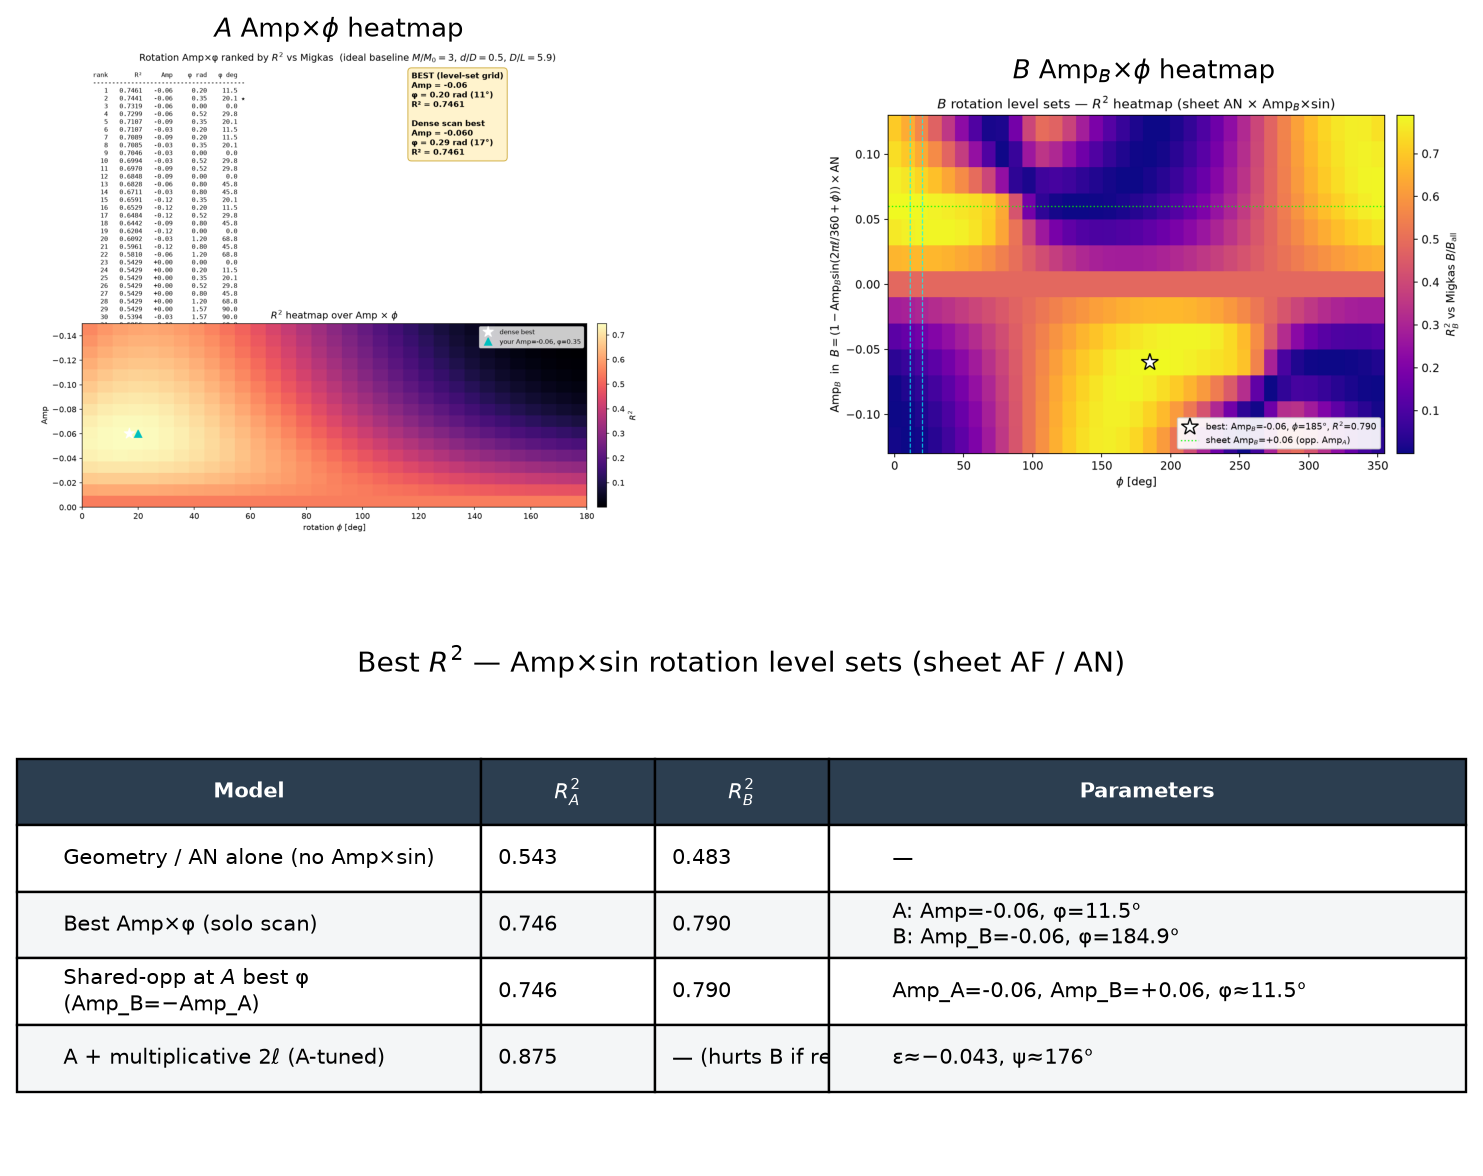
\includegraphics[width=0.85\textwidth]{R2_table_best_A_B_with_heatmaps.png}
\caption{$R^2$ tables / Amp--$\phi$ heatmaps for $A$ and $B$ under the
Amp$\times\sin$ scan.}
\label{fig:R2heat}
\end{figure}

\begin{figure}[ht]
\centering
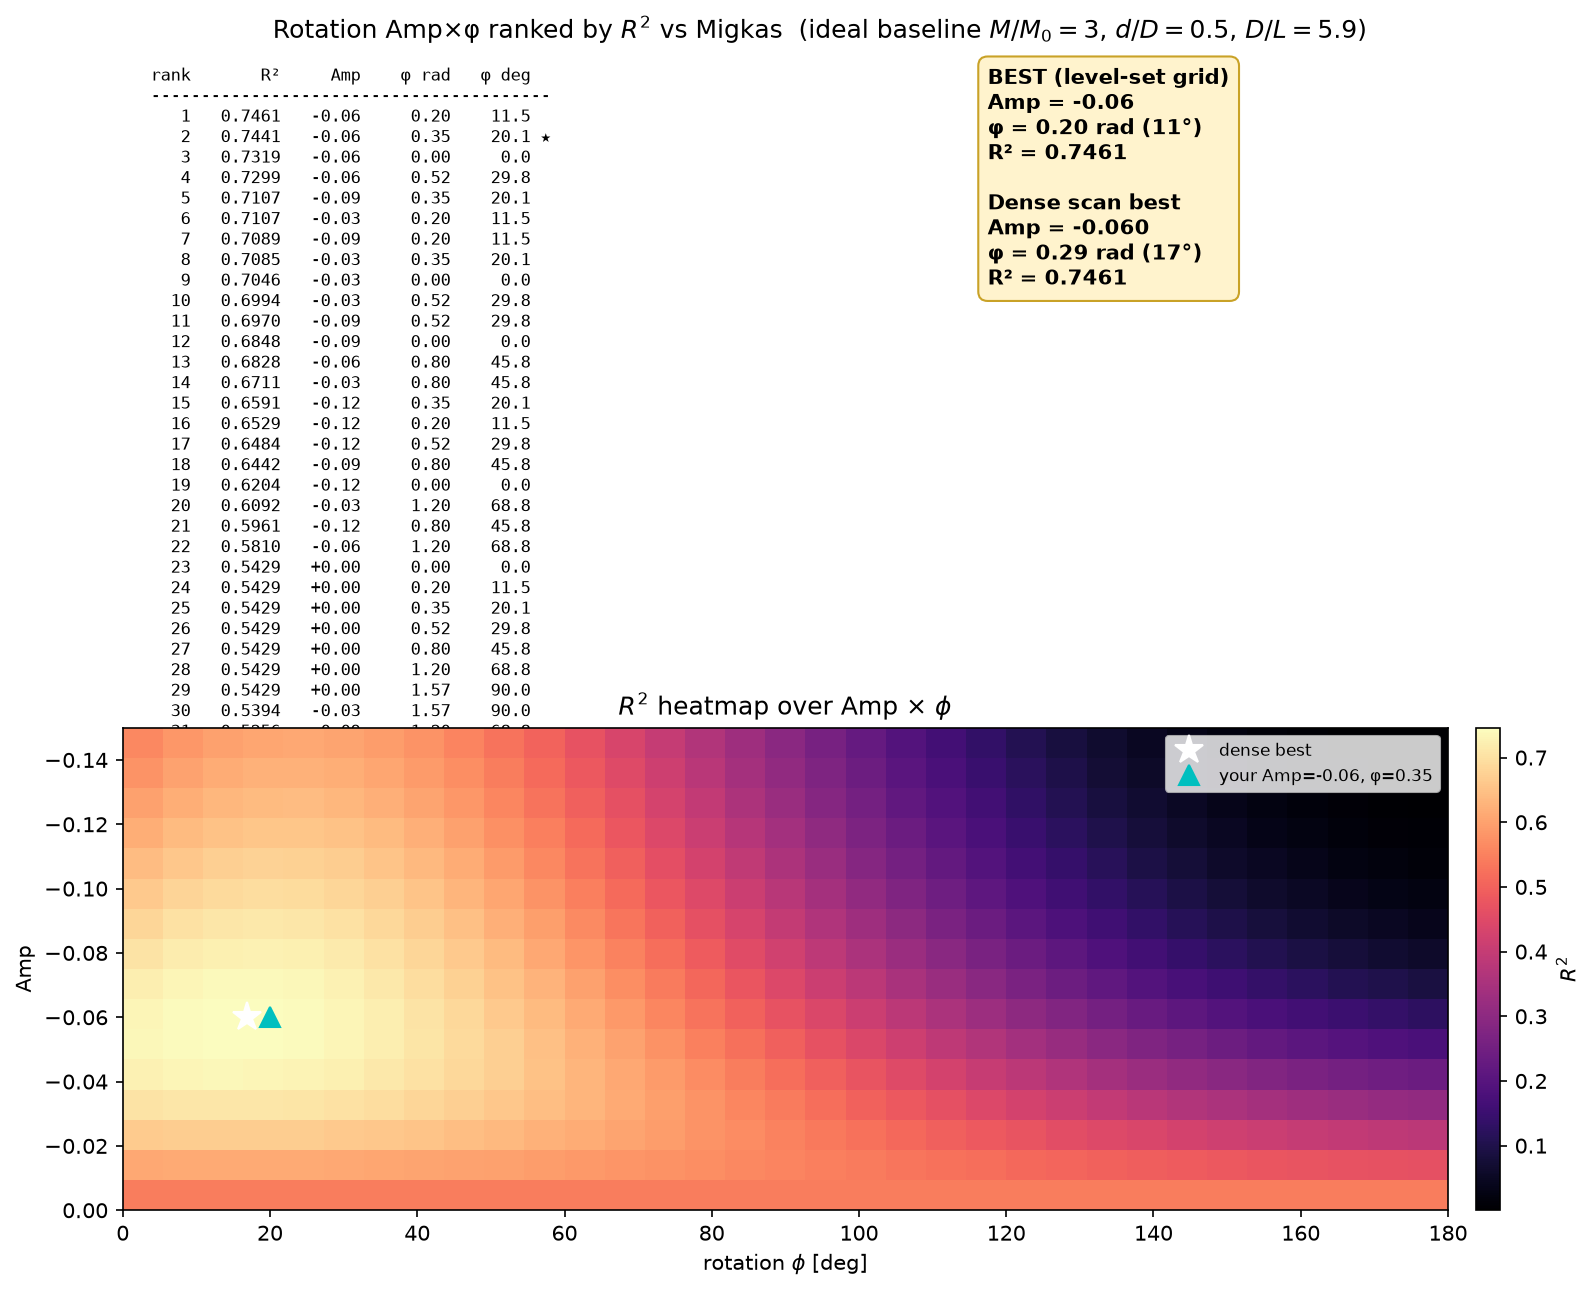
\includegraphics[width=0.88\textwidth]{rotation_Amp_phi_R2_ranked.png}
\caption{Ranked Amp--$\phi$ scan for $R^2_A$ (peak near Amp$=-0.06$,
$\phi\approx11.5^\circ$).}
\label{fig:R2rank}
\end{figure}

\begin{figure}[ht]
\centering
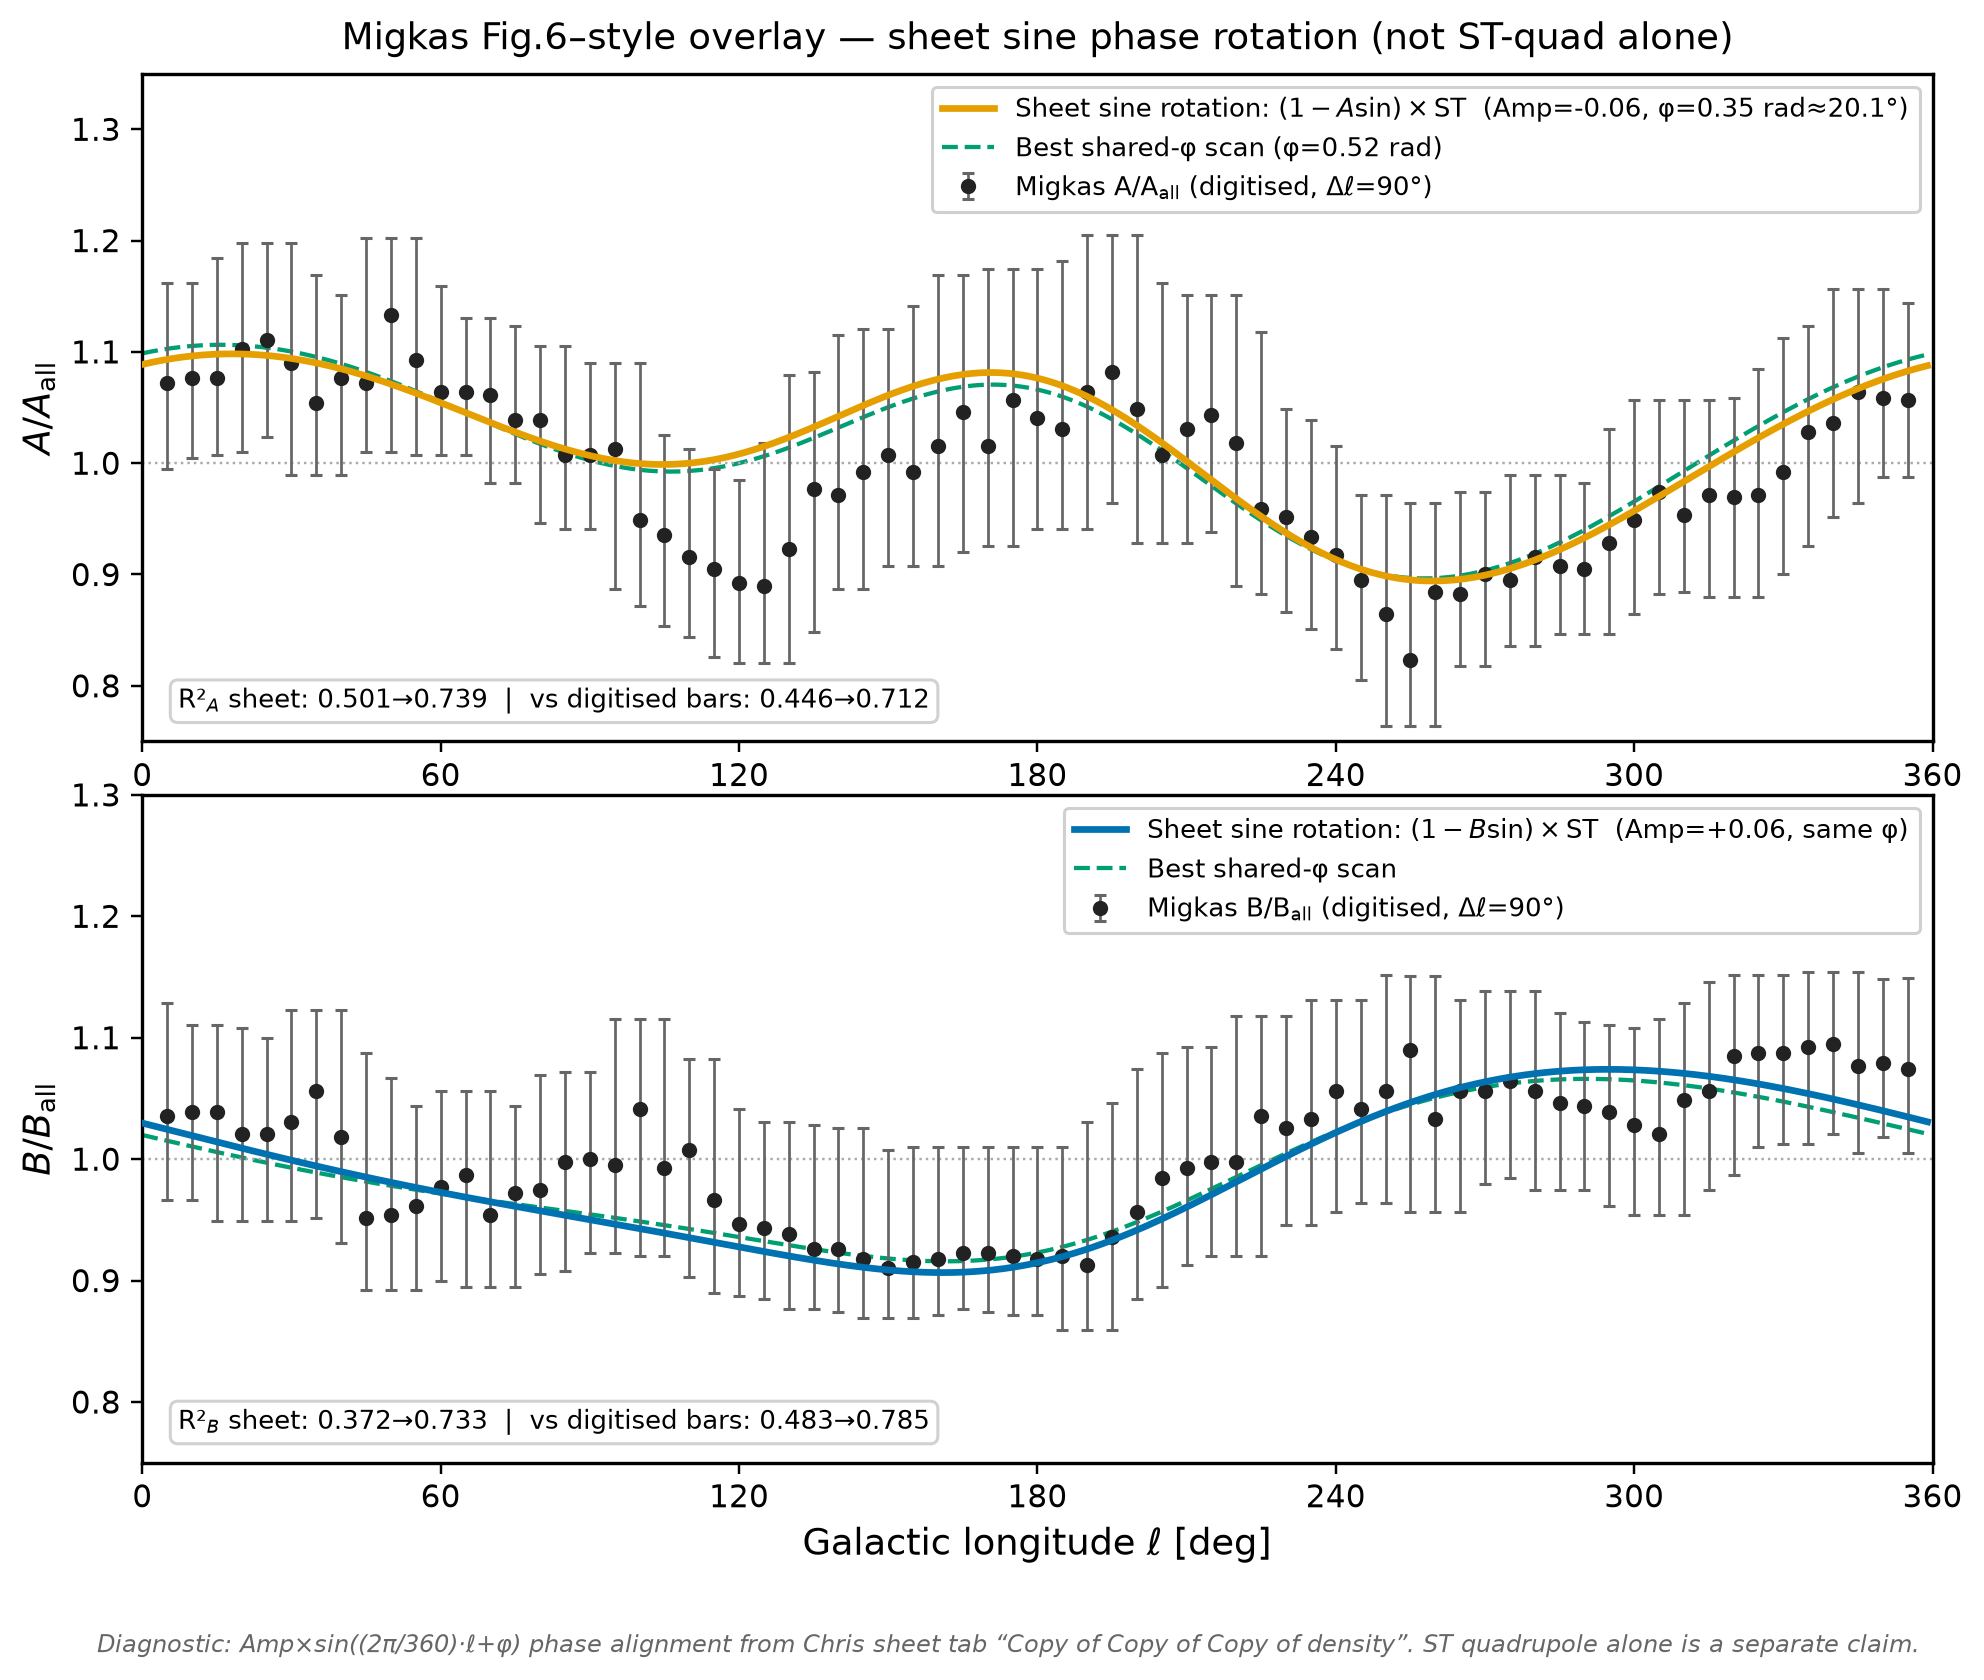
\includegraphics[width=0.92\textwidth]{migkas_bars_rotation_overlay.png}
\caption{Migkas bars with Amp$\times\sin$ rotation overlay (sheet-style diagnostic).}
\label{fig:bars}
\end{figure}

%======================================================================
\section{Residuals after rotation}
\label{sec:resid_after}

After Amp$\times\sin$, residuals shrink but retain structure
(Fig.~\ref{fig:resid_after}). The companion panel with a $\sin/\cos$ guide
(Fig.~\ref{fig:resid_sincos}) motivates the $2\ell$ layer of
Sec.~\ref{sec:2ell}.

\begin{figure}[ht]
\centering
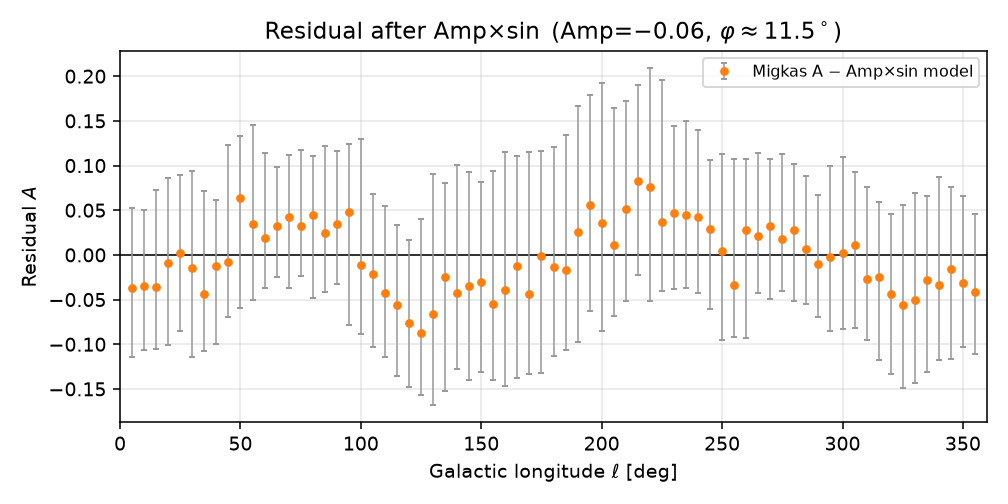
\includegraphics[width=0.92\textwidth]{residual_after_rotation.png}
\caption{Residual after Amp$\times\sin$
(Amp$=-0.06$, $\phi\approx11.5^\circ$): Migkas $A$ minus rotated model
(on-disk Amp$\times\sin$ chain).}
\label{fig:resid_after}
\end{figure}

\begin{figure}[ht]
\centering
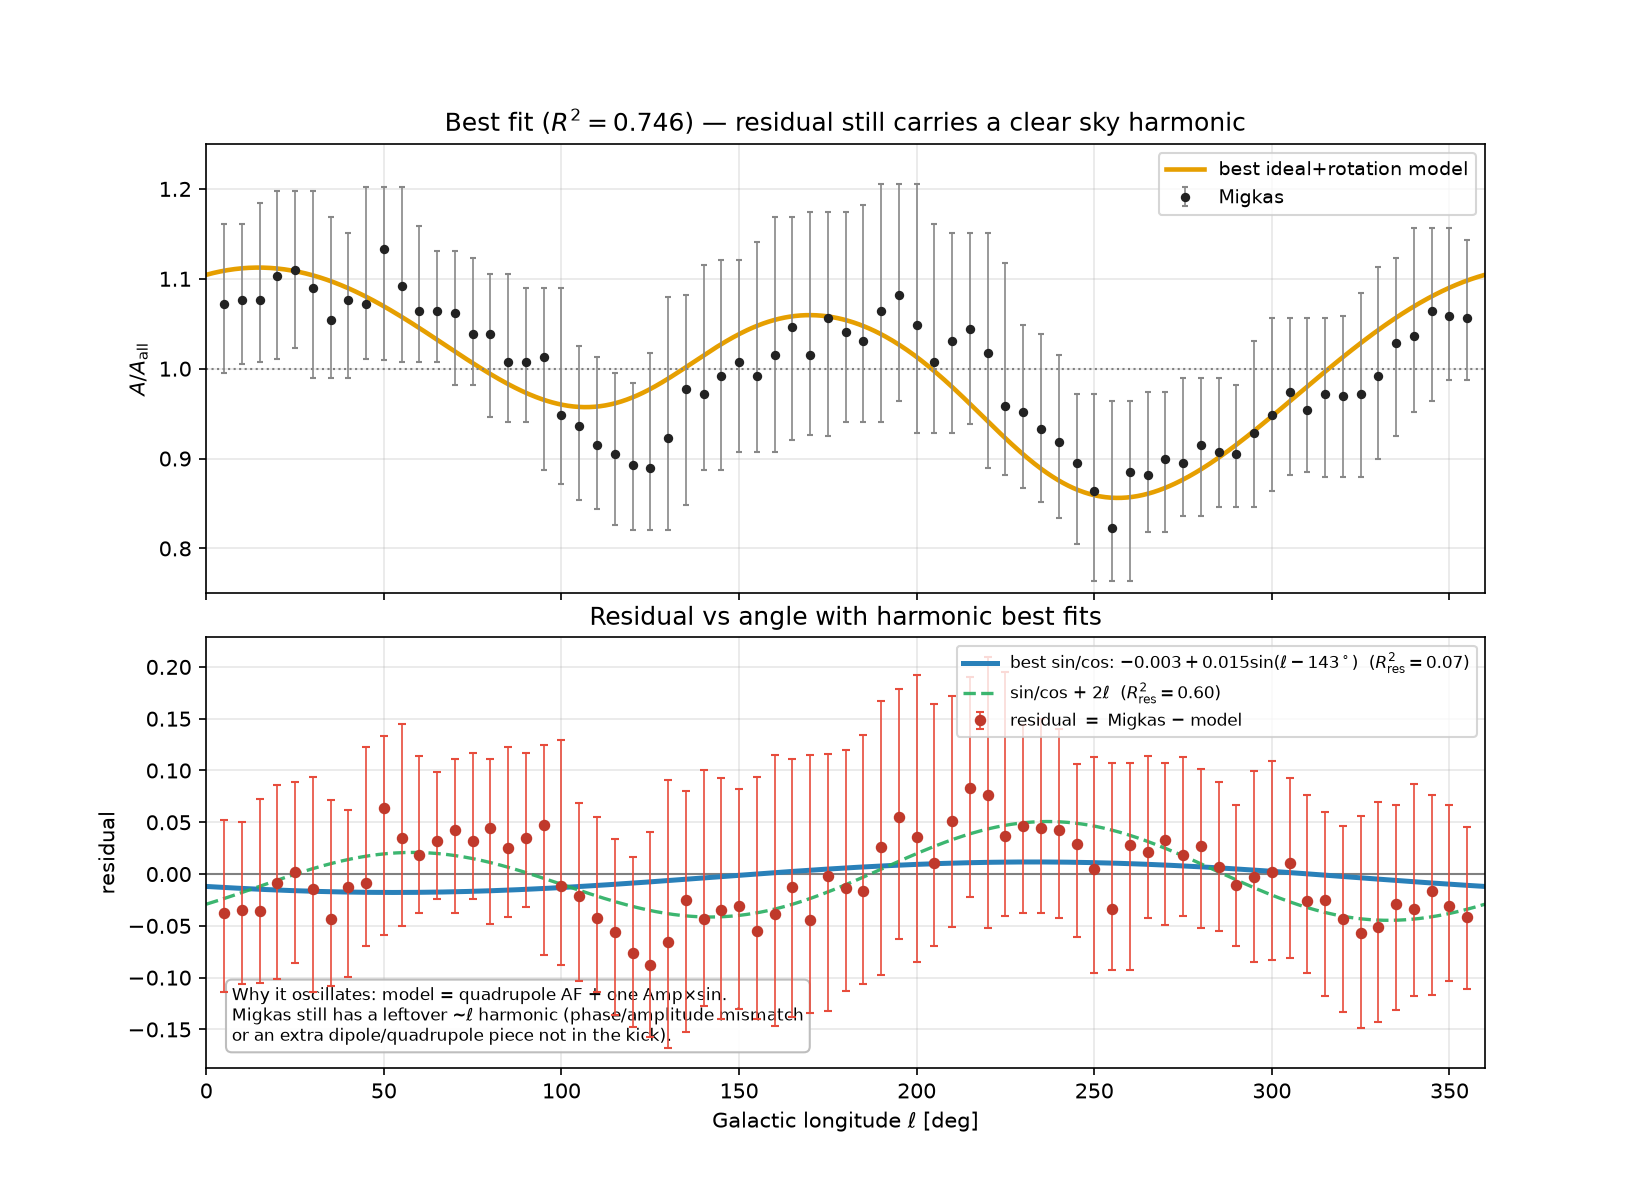
\includegraphics[width=0.92\textwidth]{best_fit_residual_vs_angle_with_sincos.png}
\caption{Post-rotation residual versus $\ell$ with $\sin/\cos$ guide curves
(existing fit product; used as input to the $2\ell$ multiplier).}
\label{fig:resid_sincos}
\end{figure}

%======================================================================
\section{$2\ell$ residual}
\label{sec:2ell}

A multiplicative residual layer tuned on $A$,
\begin{equation}
A_{2\ell}(\ell)
=
A_{\mathrm{rot}}(\ell)\,\bigl[1+\varepsilon\cos(2\ell+\psi)\bigr],
\end{equation}
with on-disk best values from \texttt{best\_fit\_2ell\_multiplier.npz}:
\begin{equation}
\varepsilon\approx-0.043,\qquad
\psi\approx176^\circ,\qquad
R^2_A\approx0.875
\end{equation}
(RMSE $0.038\to0.029$ on that chain). This is phenomenological: it absorbs
leftover quadrupole-like structure after geometry + Amp$\times\sin$.

\begin{figure}[ht]
\centering
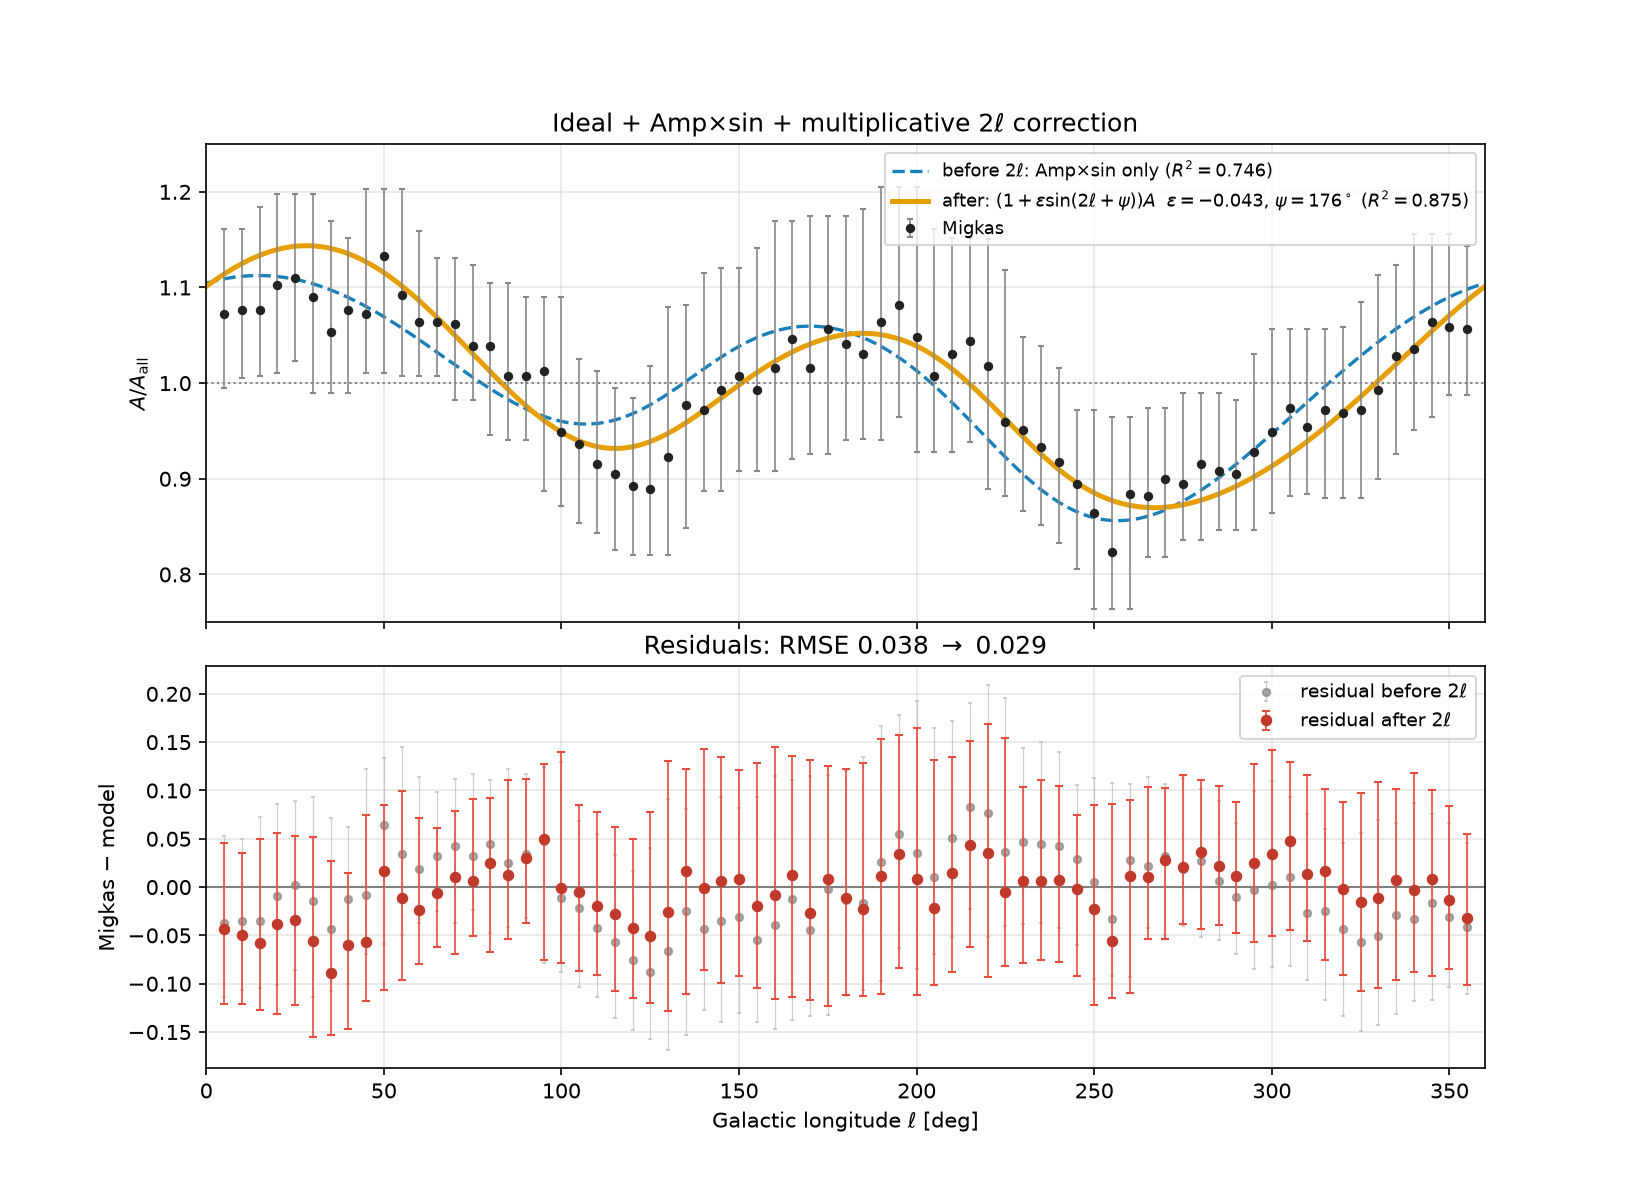
\includegraphics[width=0.90\textwidth]{best_fit_with_2ell_multiplier.png}
\caption{Best-fit Amp$\times\sin$ model with multiplicative $2\ell$ layer on
$A$ ($R^2_A\approx0.875$).}
\label{fig:2ell}
\end{figure}

\begin{figure}[ht]
\centering
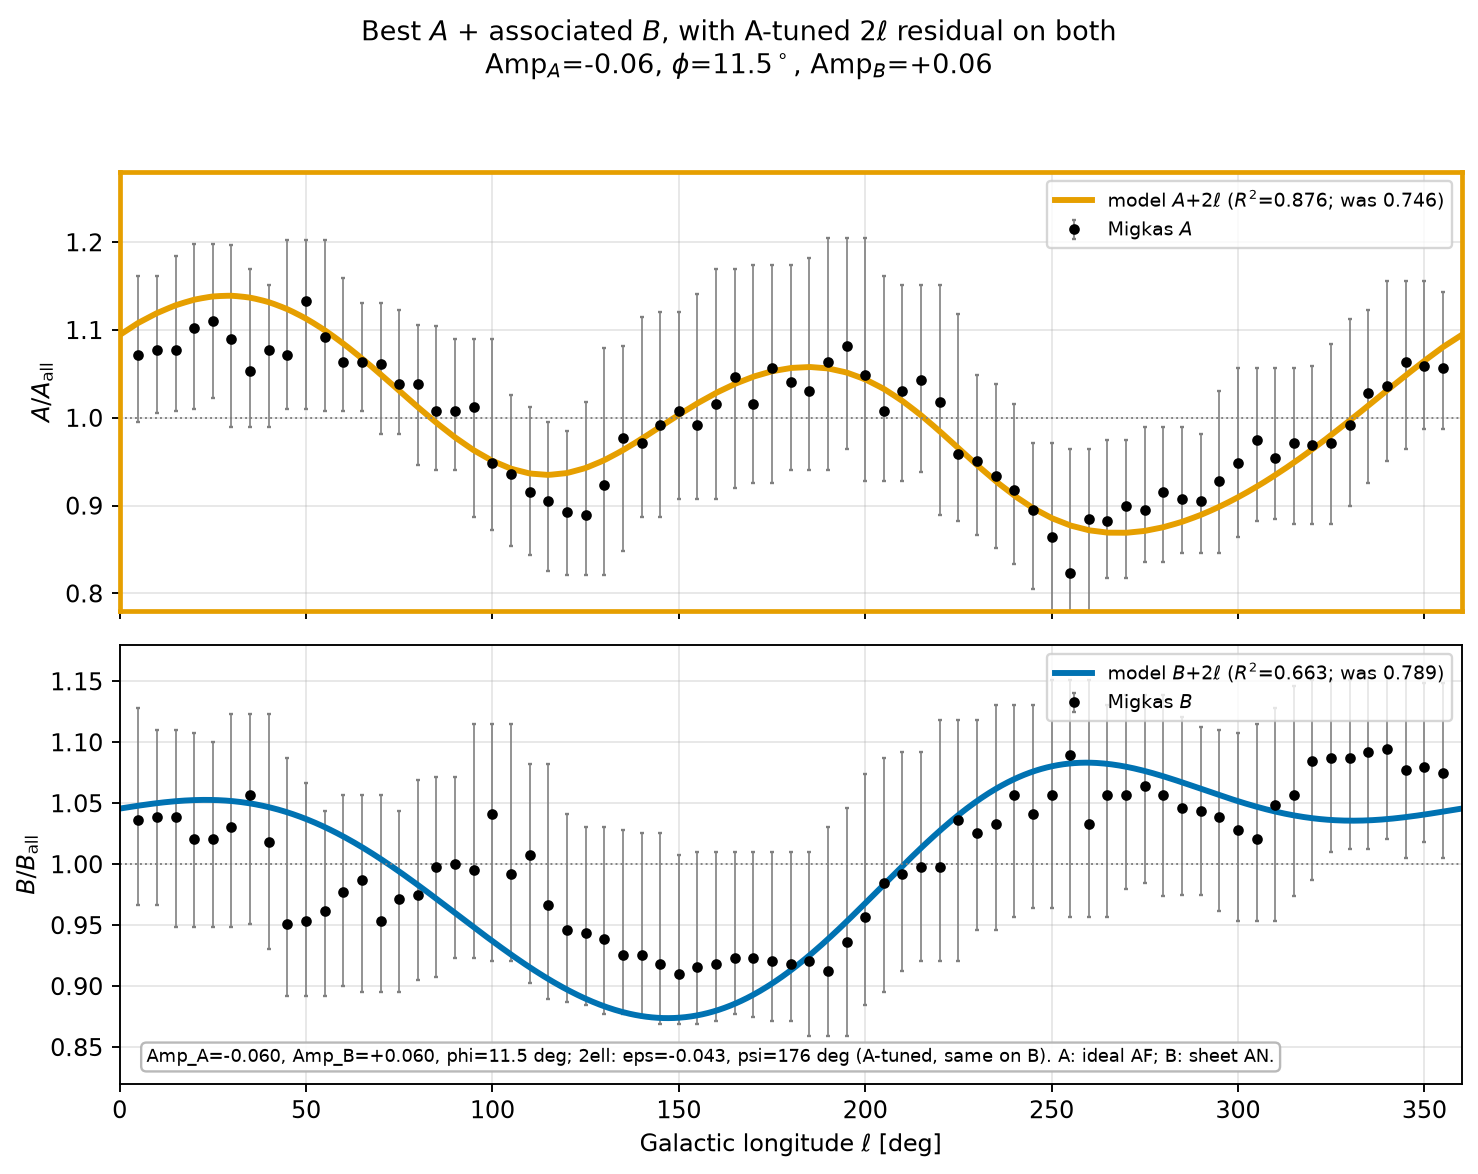
\includegraphics[width=0.90\textwidth]{best_A_vs_angle_with_associated_B_2ell.png}
\caption{$A$-tuned $2\ell$ fit with associated $B$ shown. $B$ does not improve
the same way when the $2\ell$ layer is tuned on $A$.}
\label{fig:2ellAB}
\end{figure}

\begin{figure}[ht]
\centering
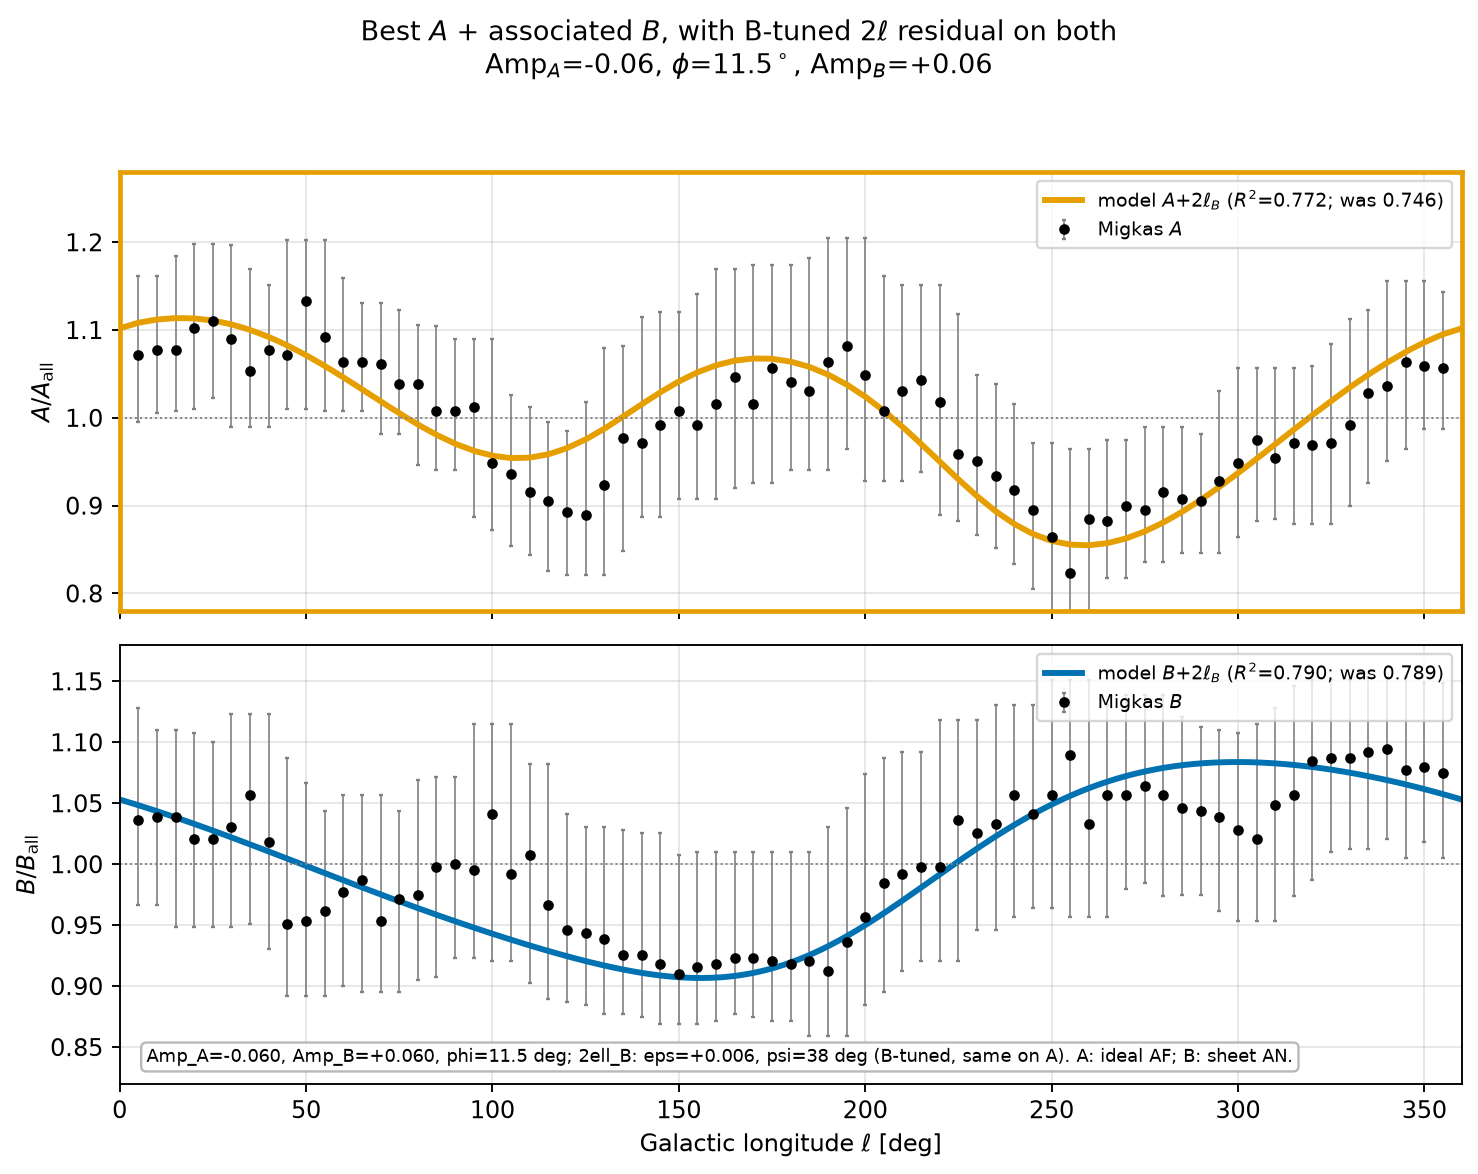
\includegraphics[width=0.90\textwidth]{best_A_vs_angle_with_associated_B_2ell_fromB.png}
\caption{Companion: $2\ell$ chain when tuned from $B$ (for contrast; $A$ is the
primary Migkas target in this note).}
\label{fig:2ellfromB}
\end{figure}

Honest summary of the $A$ ladder:
\begin{center}
\begin{tabular}{@{}lcc@{}}
\toprule
Stage & Key parameters & $R^2_A$ \\
\midrule
Geometry alone & $M/M_0=3$, $d/D=0.5$, $L\approx0.169$, $\kappa\sim0.7$ & $\approx0.543$ \\
+ Amp$\times\sin$ & Amp$=-0.06$, $\phi\approx11.46^\circ$ & $\approx0.746$ \\
+ $2\ell$ ($A$-tuned) & $\varepsilon\approx-0.043$, $\psi\approx176^\circ$ & $\approx0.875$ \\
\bottomrule
\end{tabular}
\end{center}

\begin{figure}[ht]
\centering
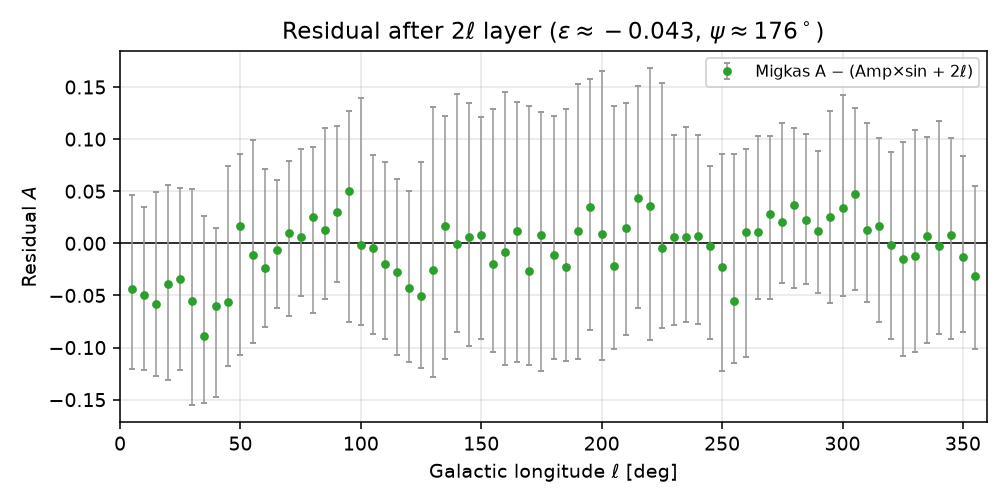
\includegraphics[width=0.88\textwidth]{residual_after_2ell.png}
\caption{Residual after the $A$-tuned $2\ell$ layer
($R^2_A\approx0.875$ on the same chain).}
\label{fig:resid_2ell}
\end{figure}

%======================================================================
\section{Migkas versus model scatter}
\label{sec:scatter}

Scatter plots make the $R^2$ meaning concrete: points lining up on $y=x$ after
the Amp$\times\sin$ (and related) adjustments.

\begin{figure}[ht]
\centering
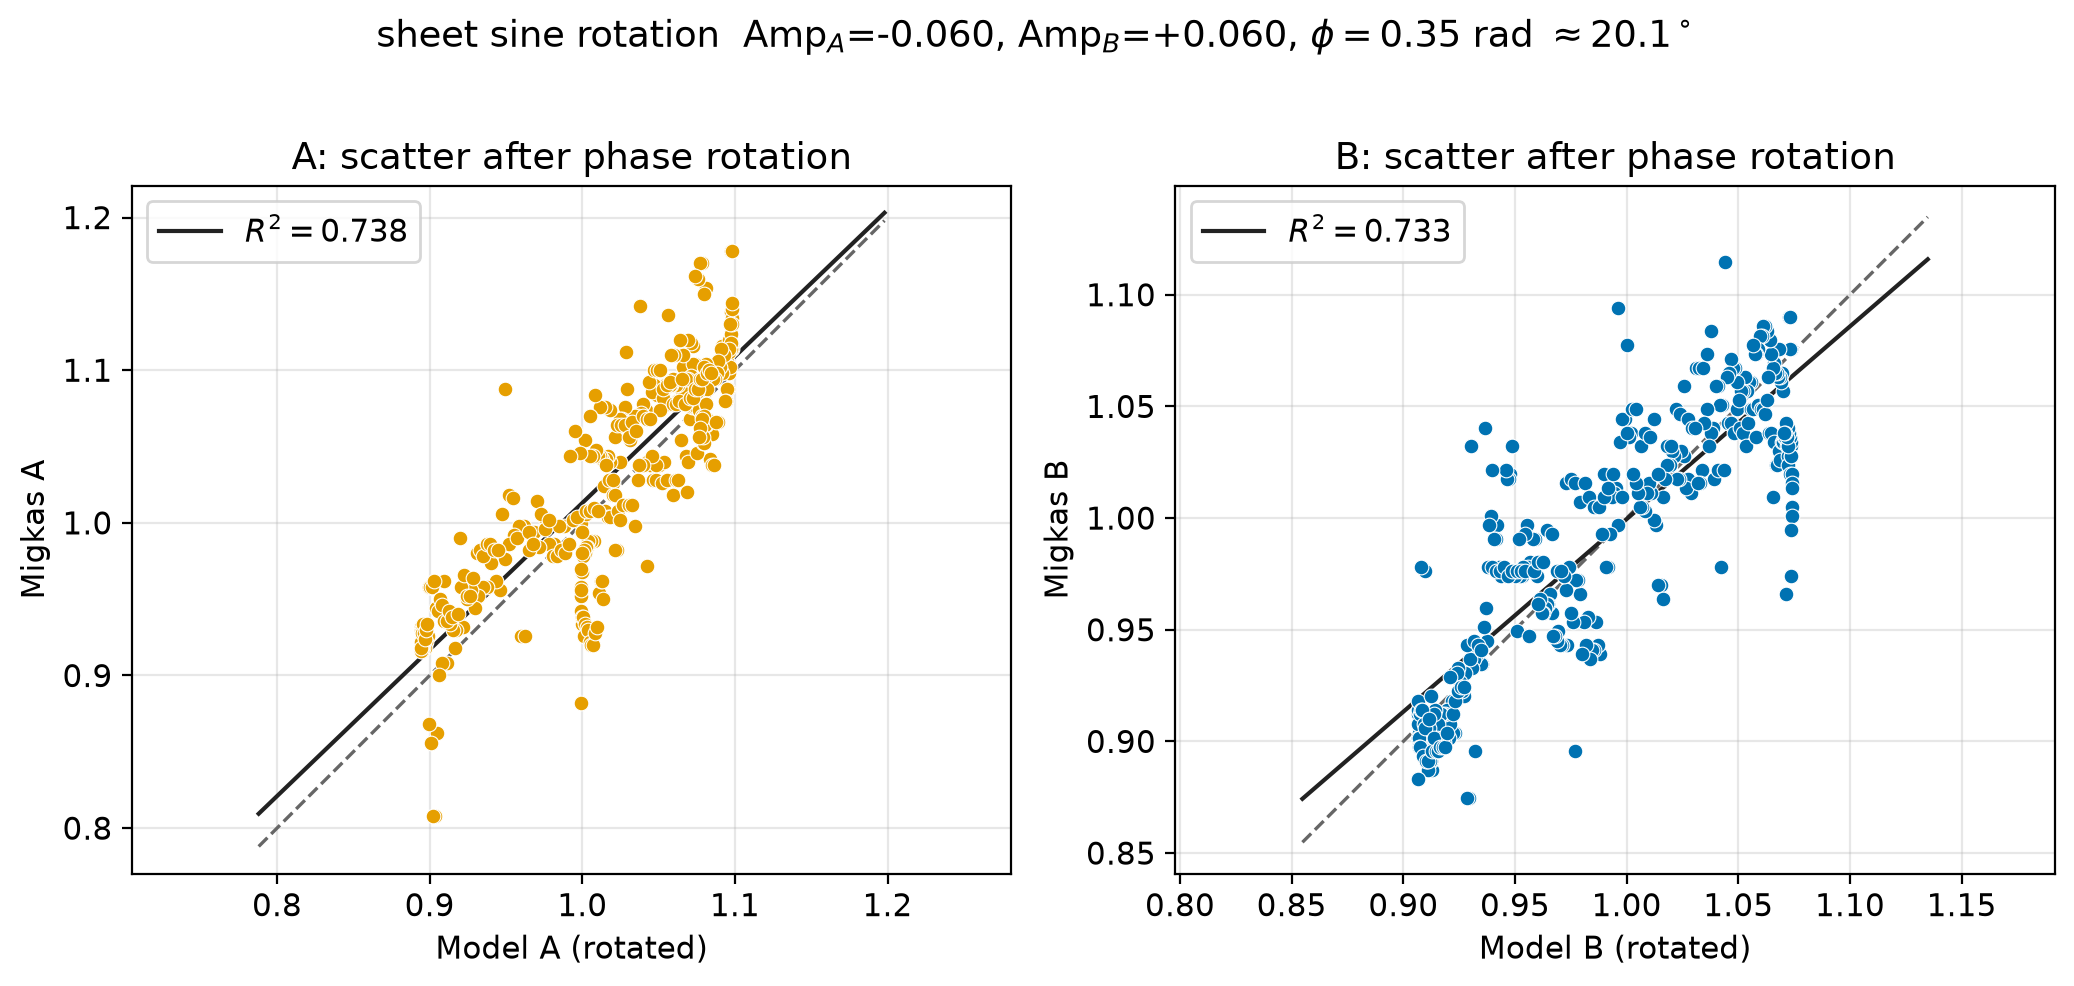
\includegraphics[width=0.72\textwidth]{migkas_sheet_scatter_amp006.png}
\caption{Migkas versus model scatter at Amp$=-0.06$ (sheet product).}
\label{fig:scatter1}
\end{figure}

\begin{figure}[ht]
\centering
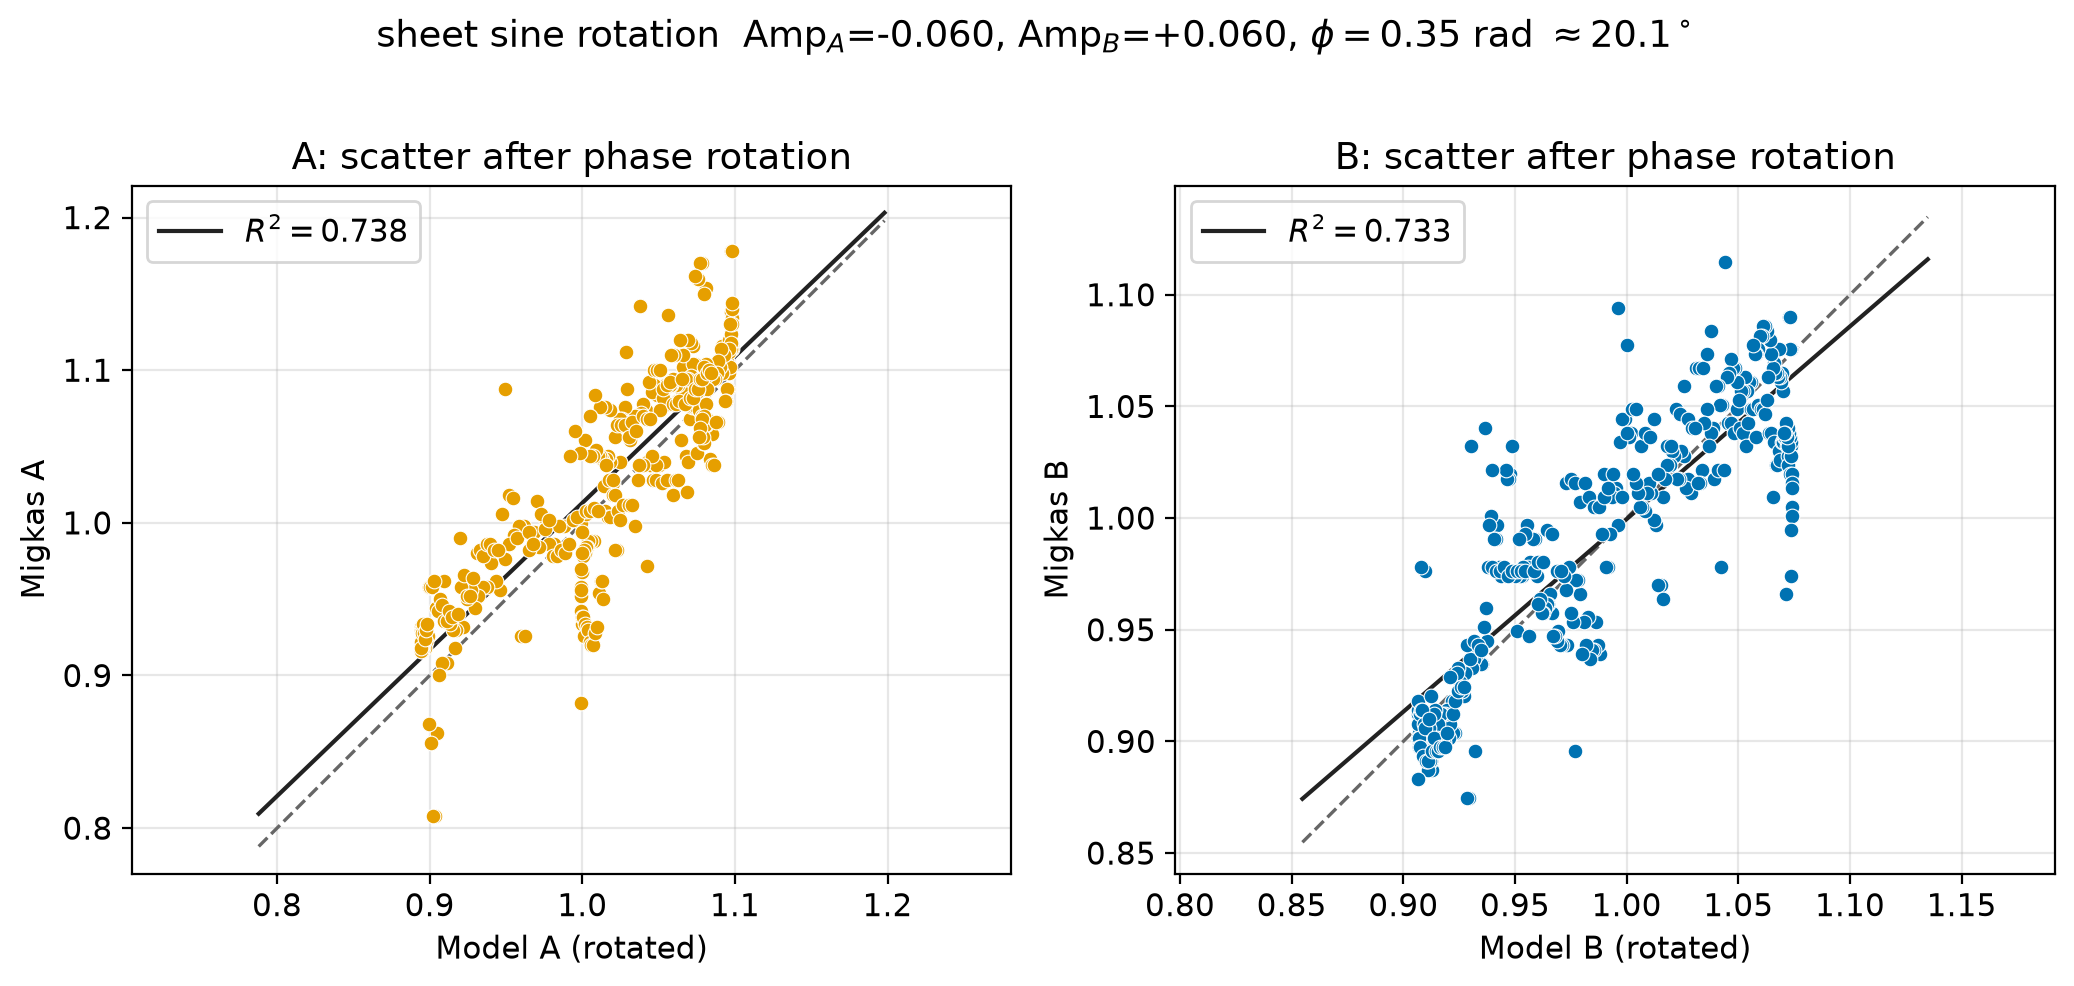
\includegraphics[width=0.72\textwidth]{migkas_bars_rotation_scatter.png}
\caption{Migkas bars versus Amp$\times\sin$ rotation model (scatter).}
\label{fig:scatter2}
\end{figure}

%======================================================================
\section{CMB dipole from shifting blackbody concentric shells}
\label{sec:cmb}

Fixsen monopole $T_0\approx2.72548\,\mathrm{K}$. Planck 2018 dipole amplitude
$A_{\mathrm{dip}}=3362.08\,\mu\mathrm{K}$, so
\begin{equation}
\Bigl(\frac{\delta T}{T}\Bigr)_{\mathrm{amp}}
\approx\frac{3362.08\times10^{-6}}{2.72548}\approx1.23\times10^{-3}.
\end{equation}
Hot--cold peak-to-peak is $\approx6.72\,\mathrm{mK}$. For blackbody intensity,
\begin{equation}
\frac{\delta T}{T}=\frac14\frac{\delta F}{F},
\end{equation}
so matching the dipole amplitude needs
$(\delta F/F)_{\mathrm{amp}}\approx4.93\times10^{-3}$.

\paragraph{Concentric-shell toy.}
Outer-shell heating offset relative to an inner shell can source a sky dipole for
an off-center observer. Scenarios 0, 2, and 4 are retained; Scenario~1 is dropped
for producing an unacceptably large shift. In the thin-shell picture,
$T_{\mathrm{in}}\approx T_{\mathrm{out}}\approx T_0$; a cavity (Kirchhoff) would
kill the dipole. Geometric flux contrast scaling as $\delta F/F\sim D/R$ implies
\begin{equation}
\frac{R}{D}\approx203
\end{equation}
to reach $(\delta F/F)\approx4.93\times10^{-3}$. That is a kinematic/flux toy, not
a radiative-transfer solution.

\begin{figure}[ht]
\centering
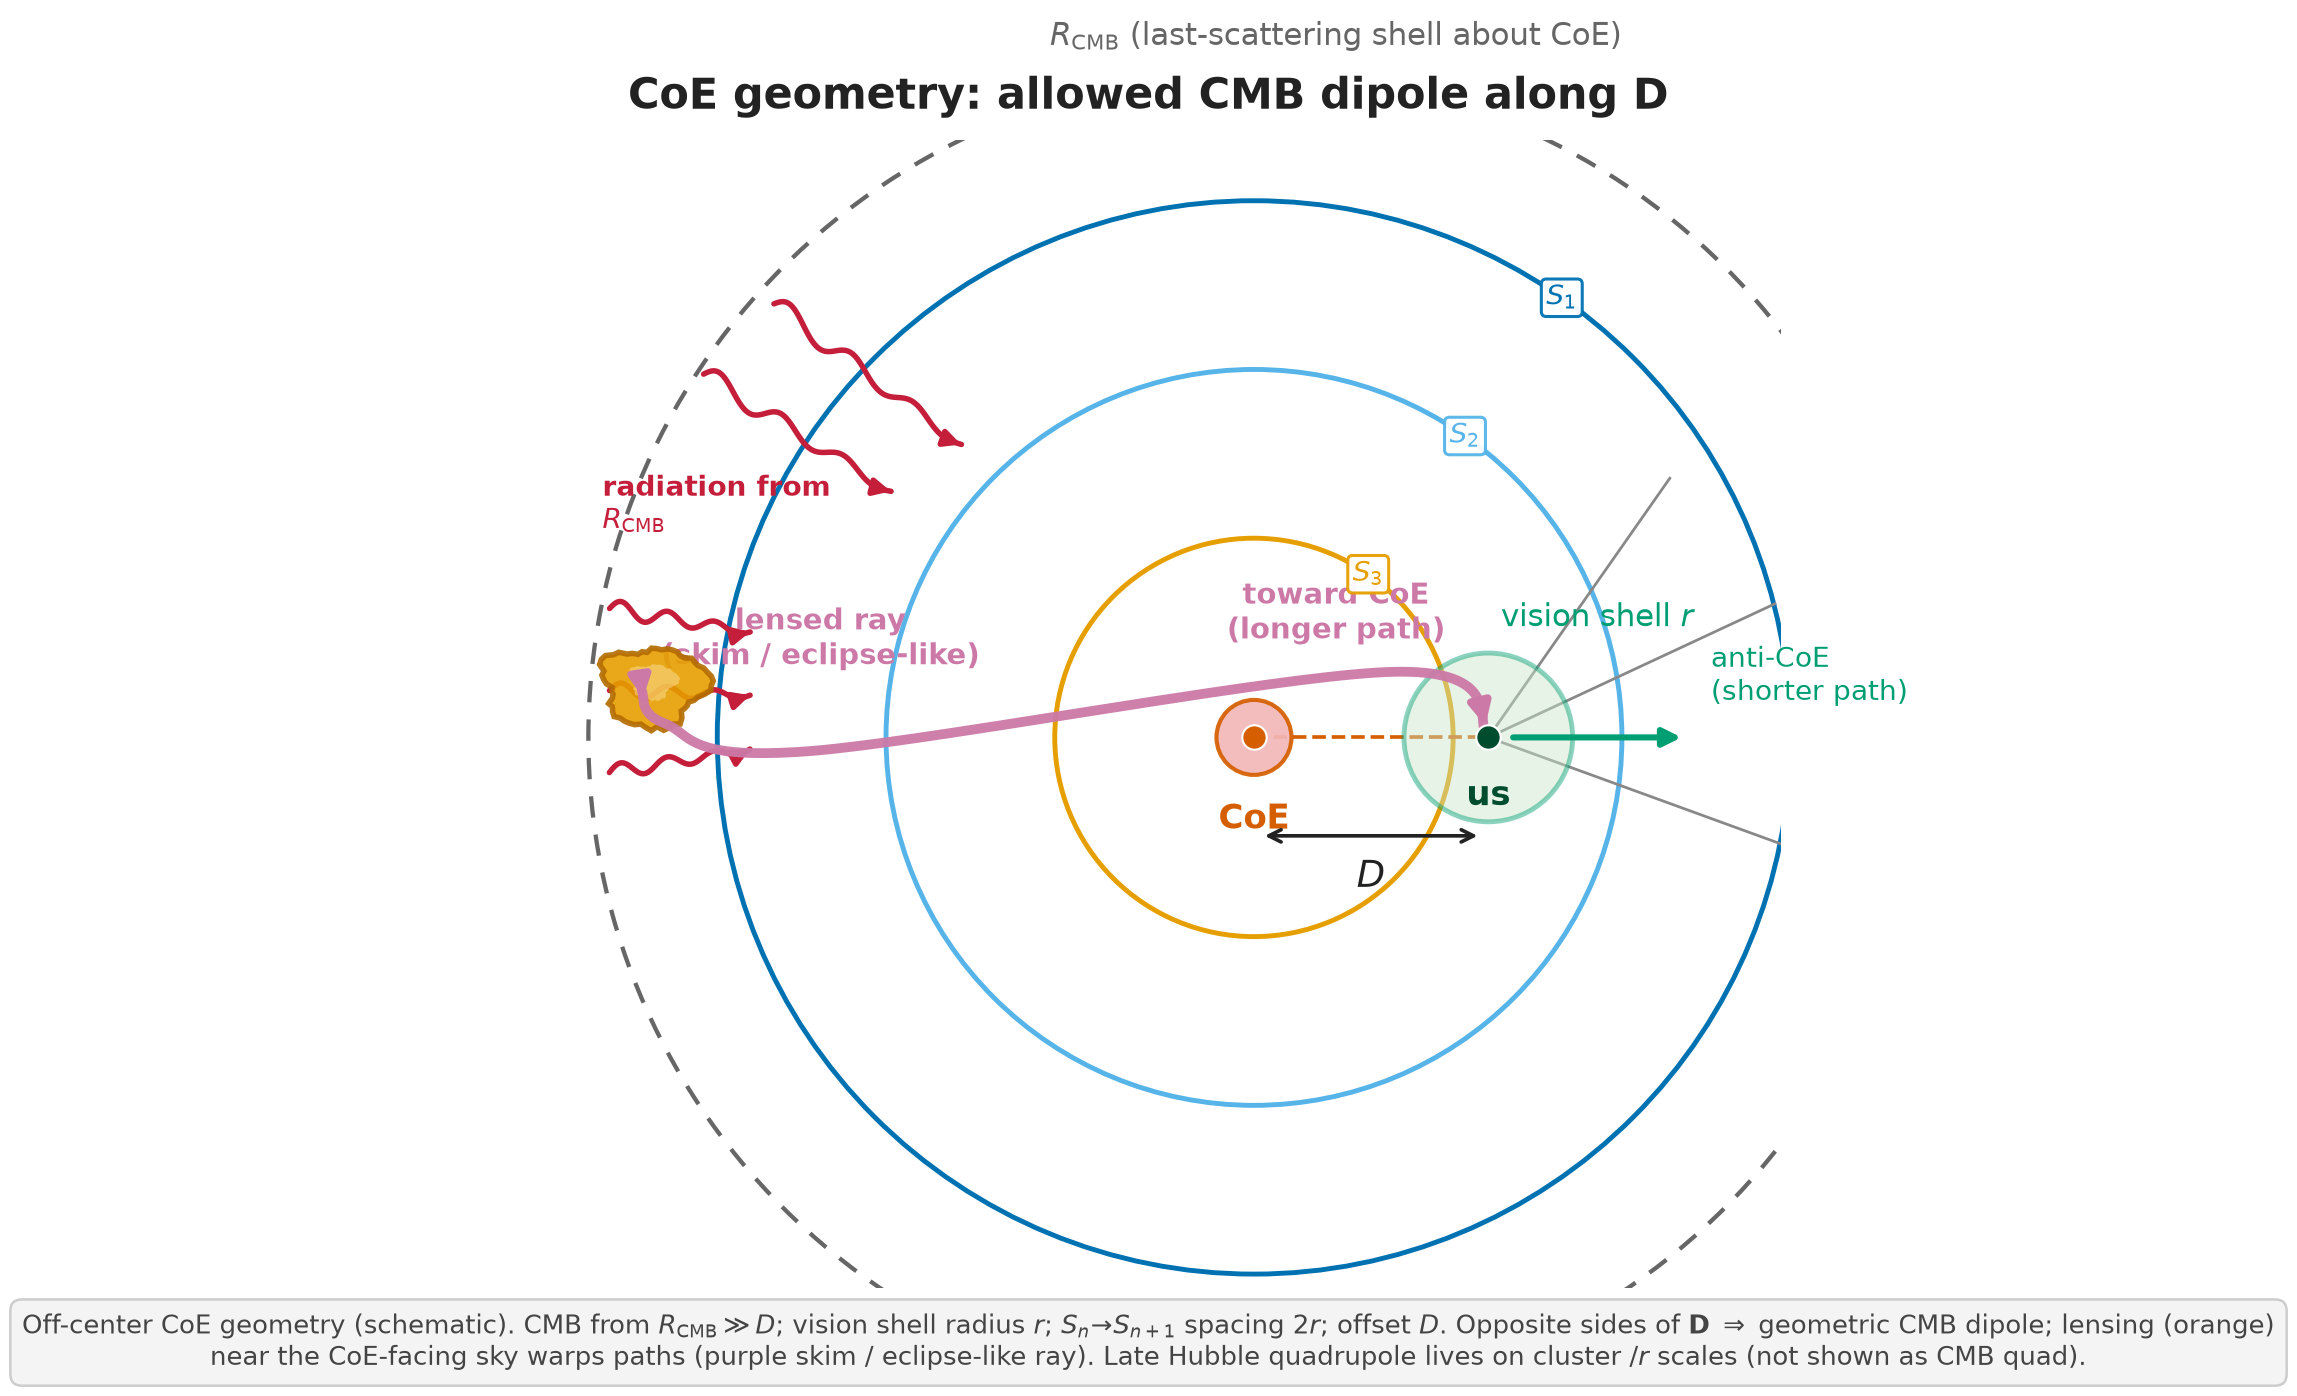
\includegraphics[width=0.88\textwidth]{coe_geometry_cmb_dipole_schematic.png}
\caption{Schematic: off-center observer inside concentric shells; outer-shell
heating offset can imprint a dipole.}
\label{fig:cmbschematic}
\end{figure}

\begin{figure}[ht]
\centering
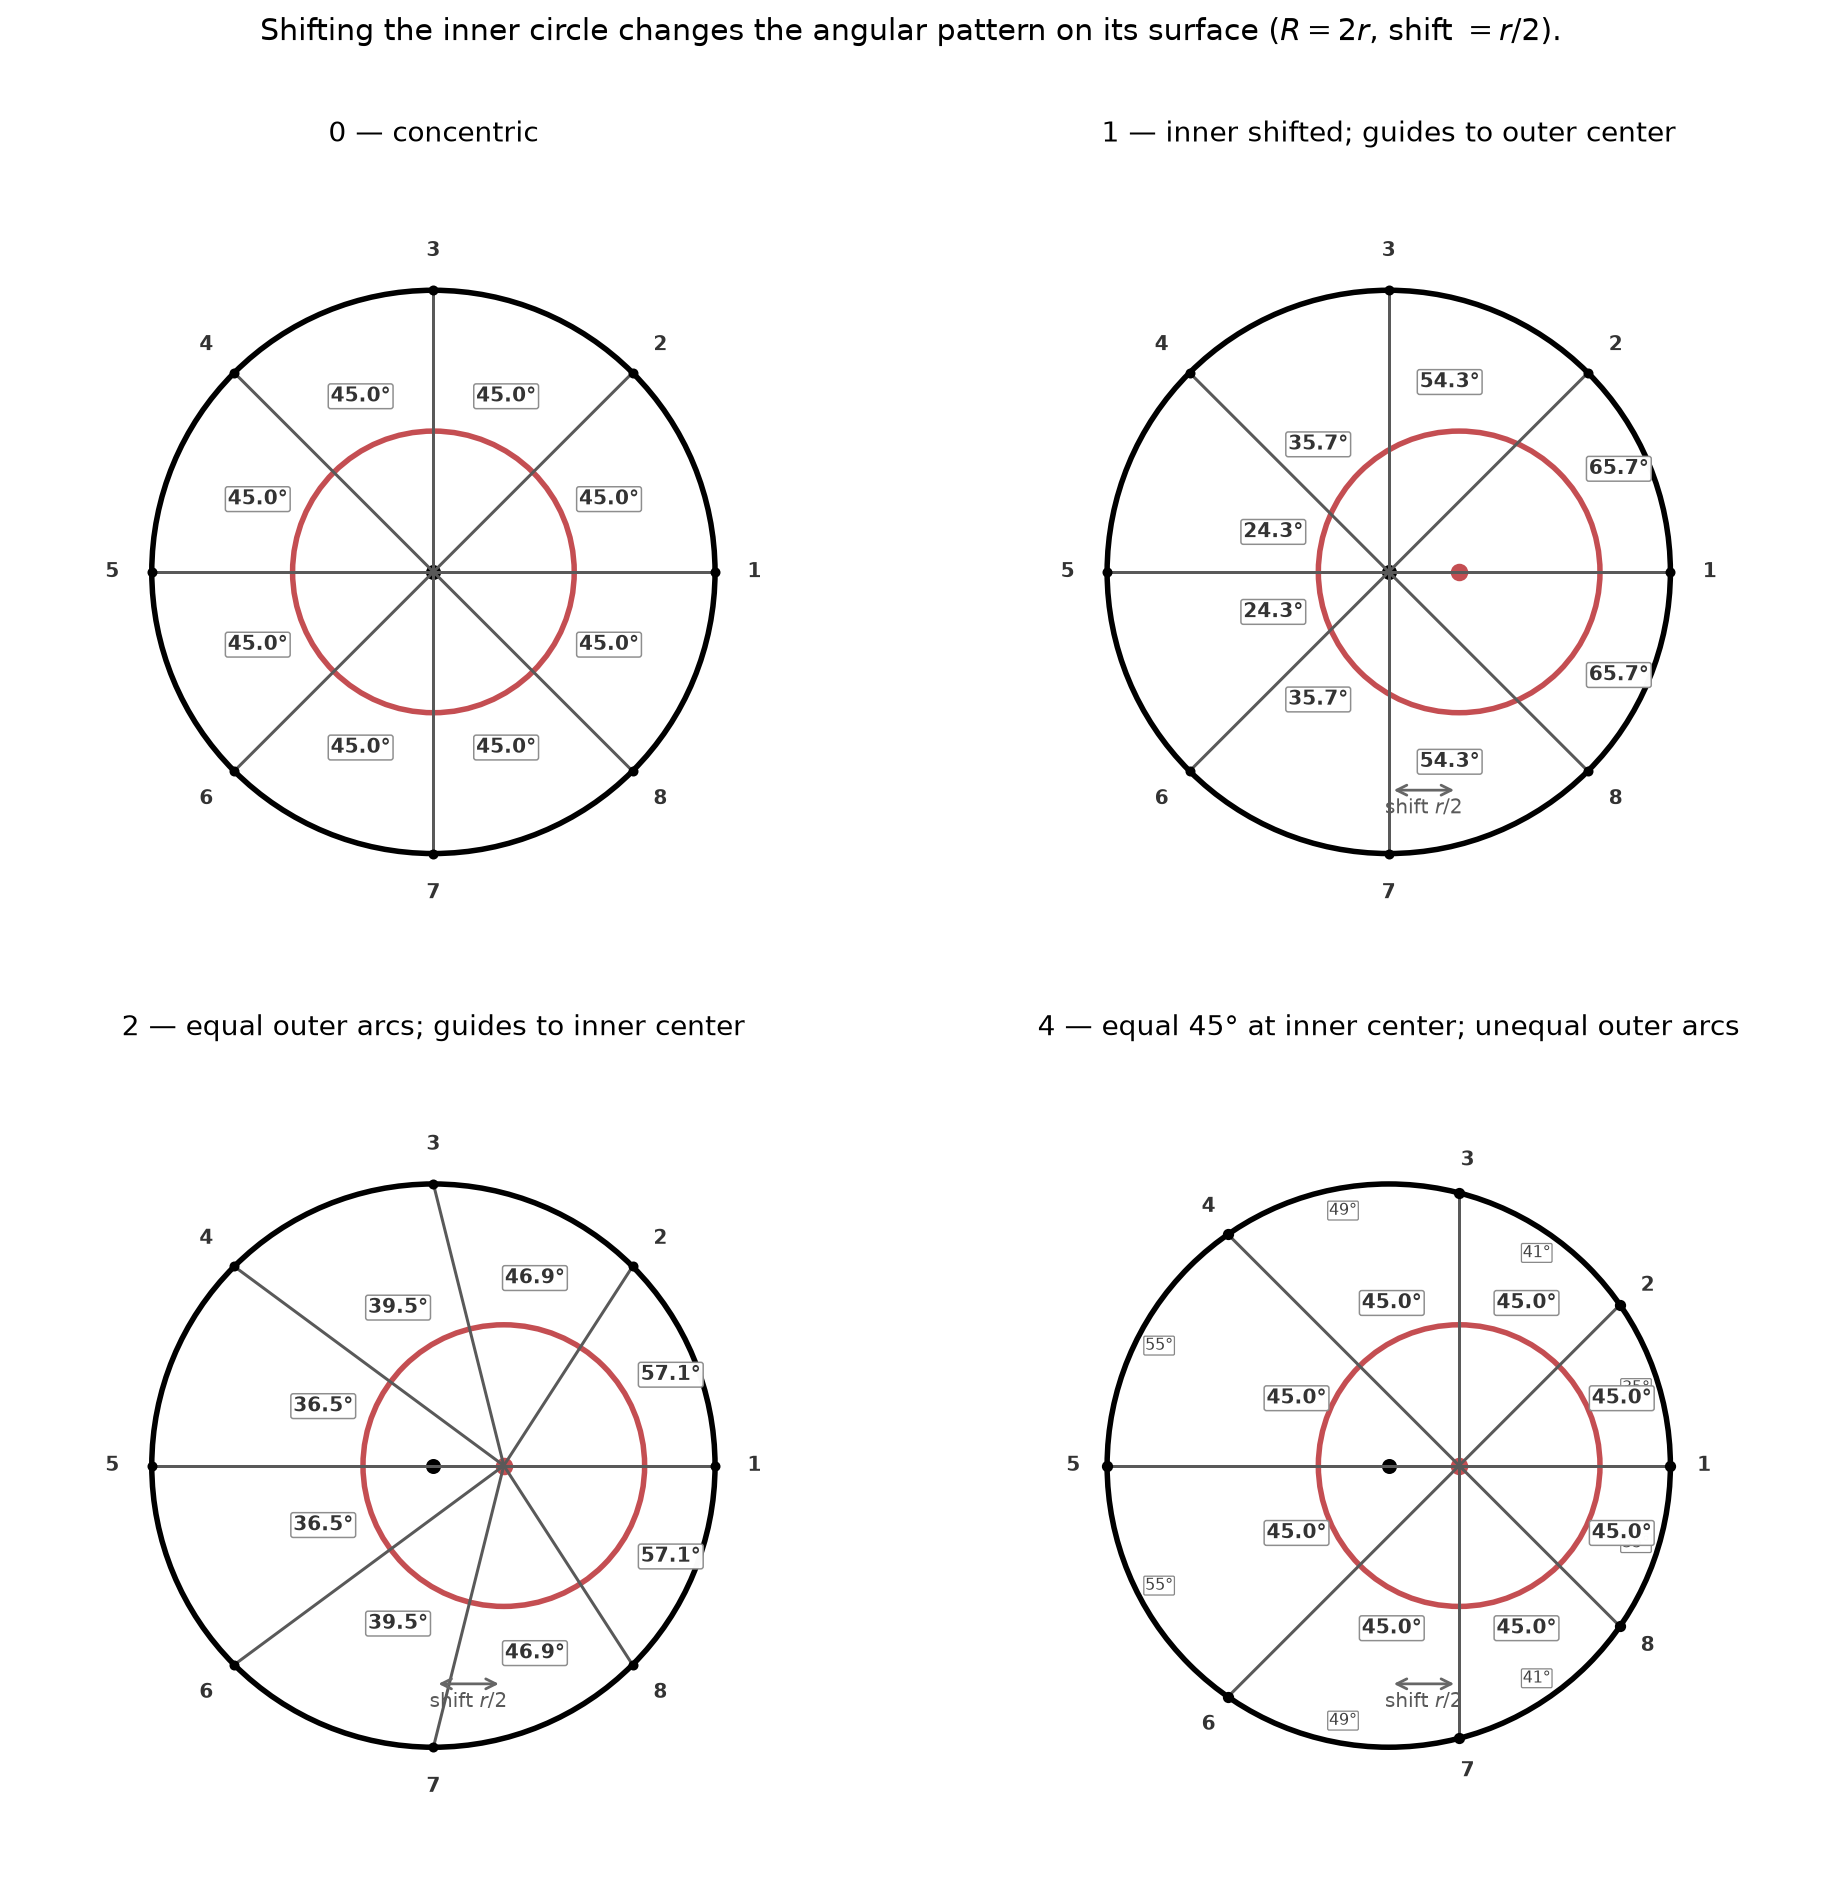
\includegraphics[width=0.92\textwidth]{four_scenarios_overview.png}
\caption{Four shell-heating scenarios overview. Scenario~1 is dropped for large
shift; Scenarios 0, 2, 4 are the working set.}
\label{fig:four}
\end{figure}

\begin{figure}[ht]
\centering
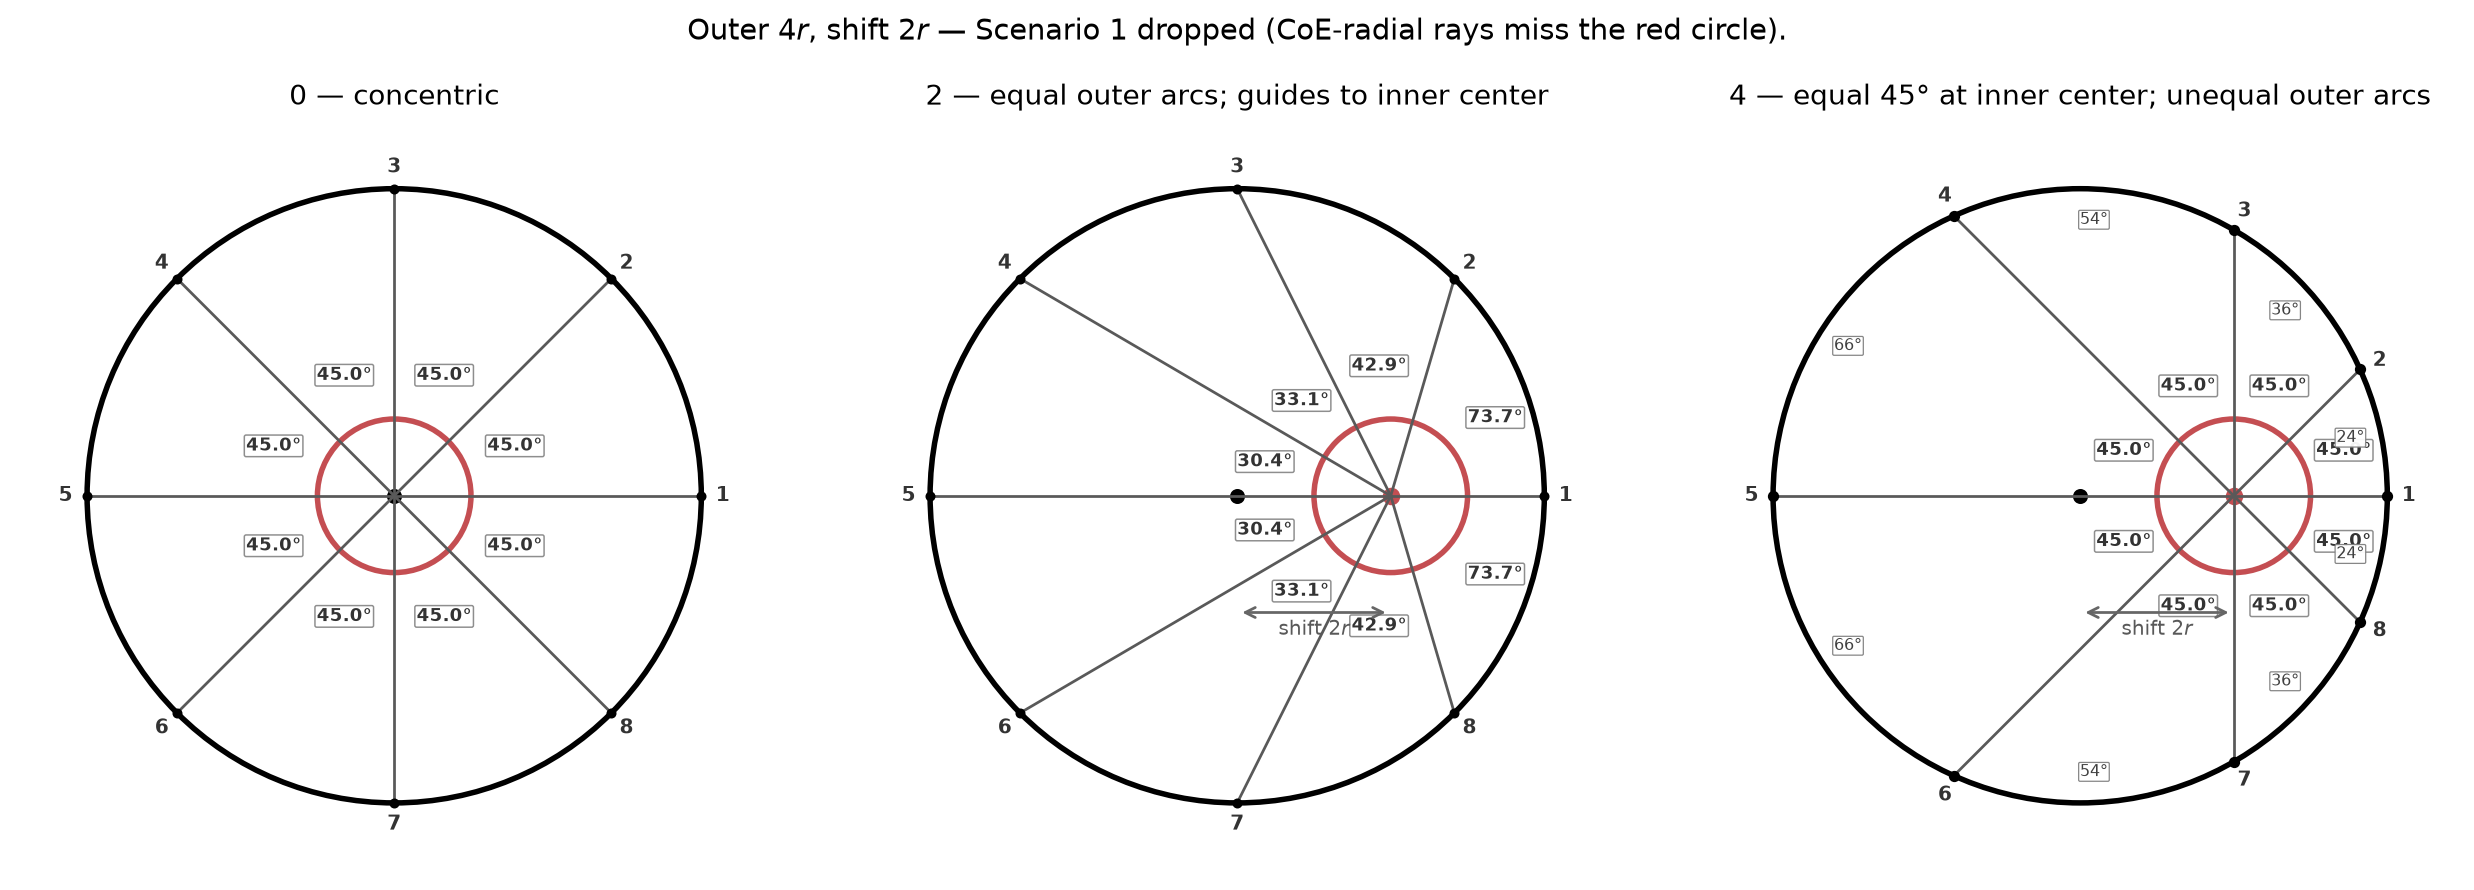
\includegraphics[width=0.92\textwidth]{scenarios_024_R4r_shift2r.png}
\caption{Scenarios 0, 2, 4 at illustrative $R=4r$, shift $2r$ (geometry demo;
CMB amplitude matching uses $R/D\sim203$).}
\label{fig:sc024}
\end{figure}

%======================================================================
\section{2D maps (Mollweide)}
\label{sec:maps}

Full-sky products in this program remain provisional. Figure~\ref{fig:moll_old}
is the existing \texttt{sky\_mollweide.png}: useful as a stage-setting sky
sketch, not a polished publication map. Figure~\ref{fig:moll_ampsin} is a
cleaner Amp$\times\sin$ \emph{dipole-proxy} Mollweide locked to the CoE axis
inferred from Amp$\times\sin$ + Planck $|b|$:
\begin{equation}
\begin{aligned}
\mathrm{CoE/cold}&\approx(258.5^\circ,+48.3^\circ),\\
\mathrm{anti\text{-}CoE/hot}&\approx(78.5^\circ,-48.3^\circ),
\end{aligned}
\end{equation}
with the usual hot/cold flip caveat relative to a pure Planck kinematic dipole
reading. This is \emph{not} a full ST+Gauss projected $A$ map---only an axis
lock for orientation.

\begin{figure}[ht]
\centering
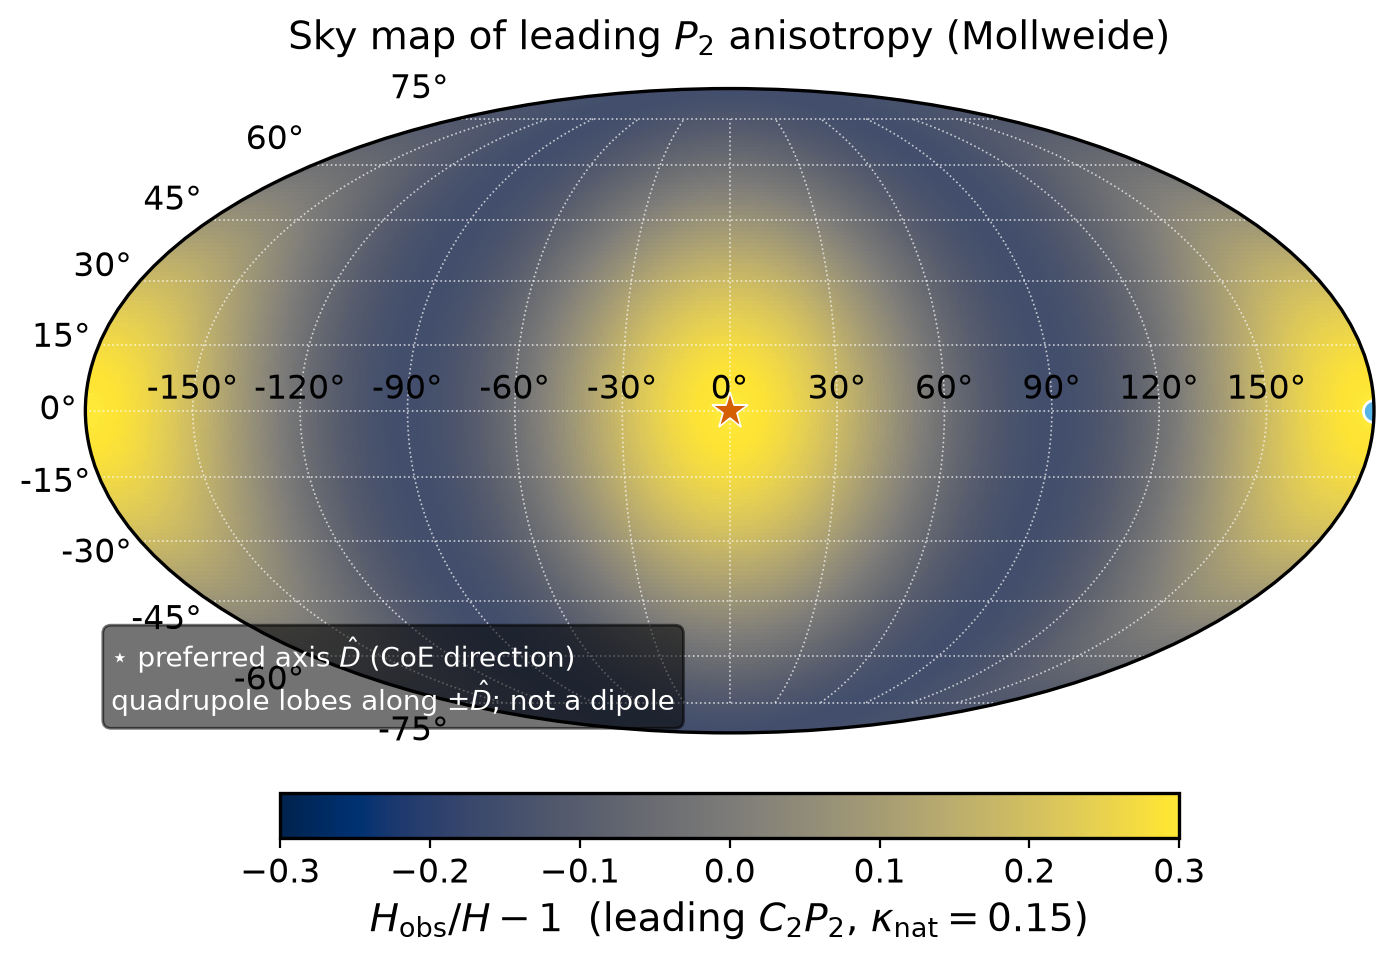
\includegraphics[width=0.88\textwidth]{sky_mollweide.png}
\caption{Existing program Mollweide (\texttt{sky\_mollweide.png}). Provisional;
included honestly as a stage-setting sky product.}
\label{fig:moll_old}
\end{figure}

\begin{figure}[ht]
\centering
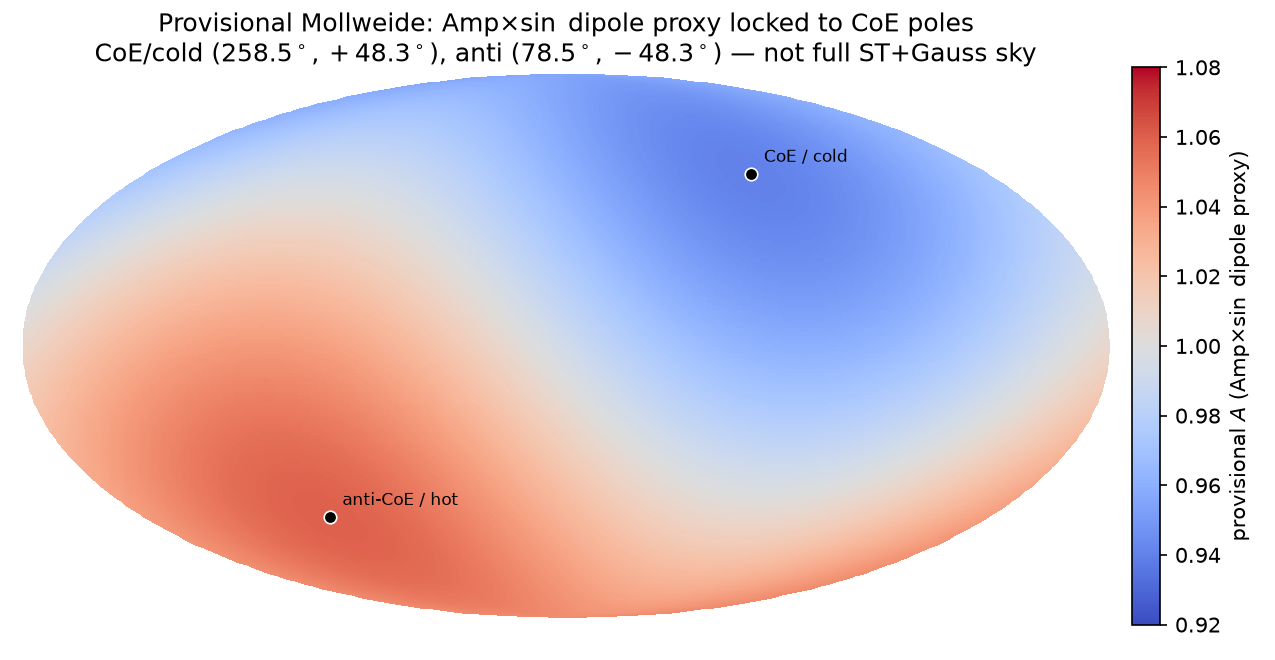
\includegraphics[width=0.92\textwidth]{mollweide_amp_sin_coe_axis.png}
\caption{Provisional Mollweide of an Amp$\times\sin$ dipole proxy with CoE poles
locked to $(258.5^\circ,+48.3^\circ)$ / $(78.5^\circ,-48.3^\circ)$.}
\label{fig:moll_ampsin}
\end{figure}

\begin{figure}[ht]
\centering
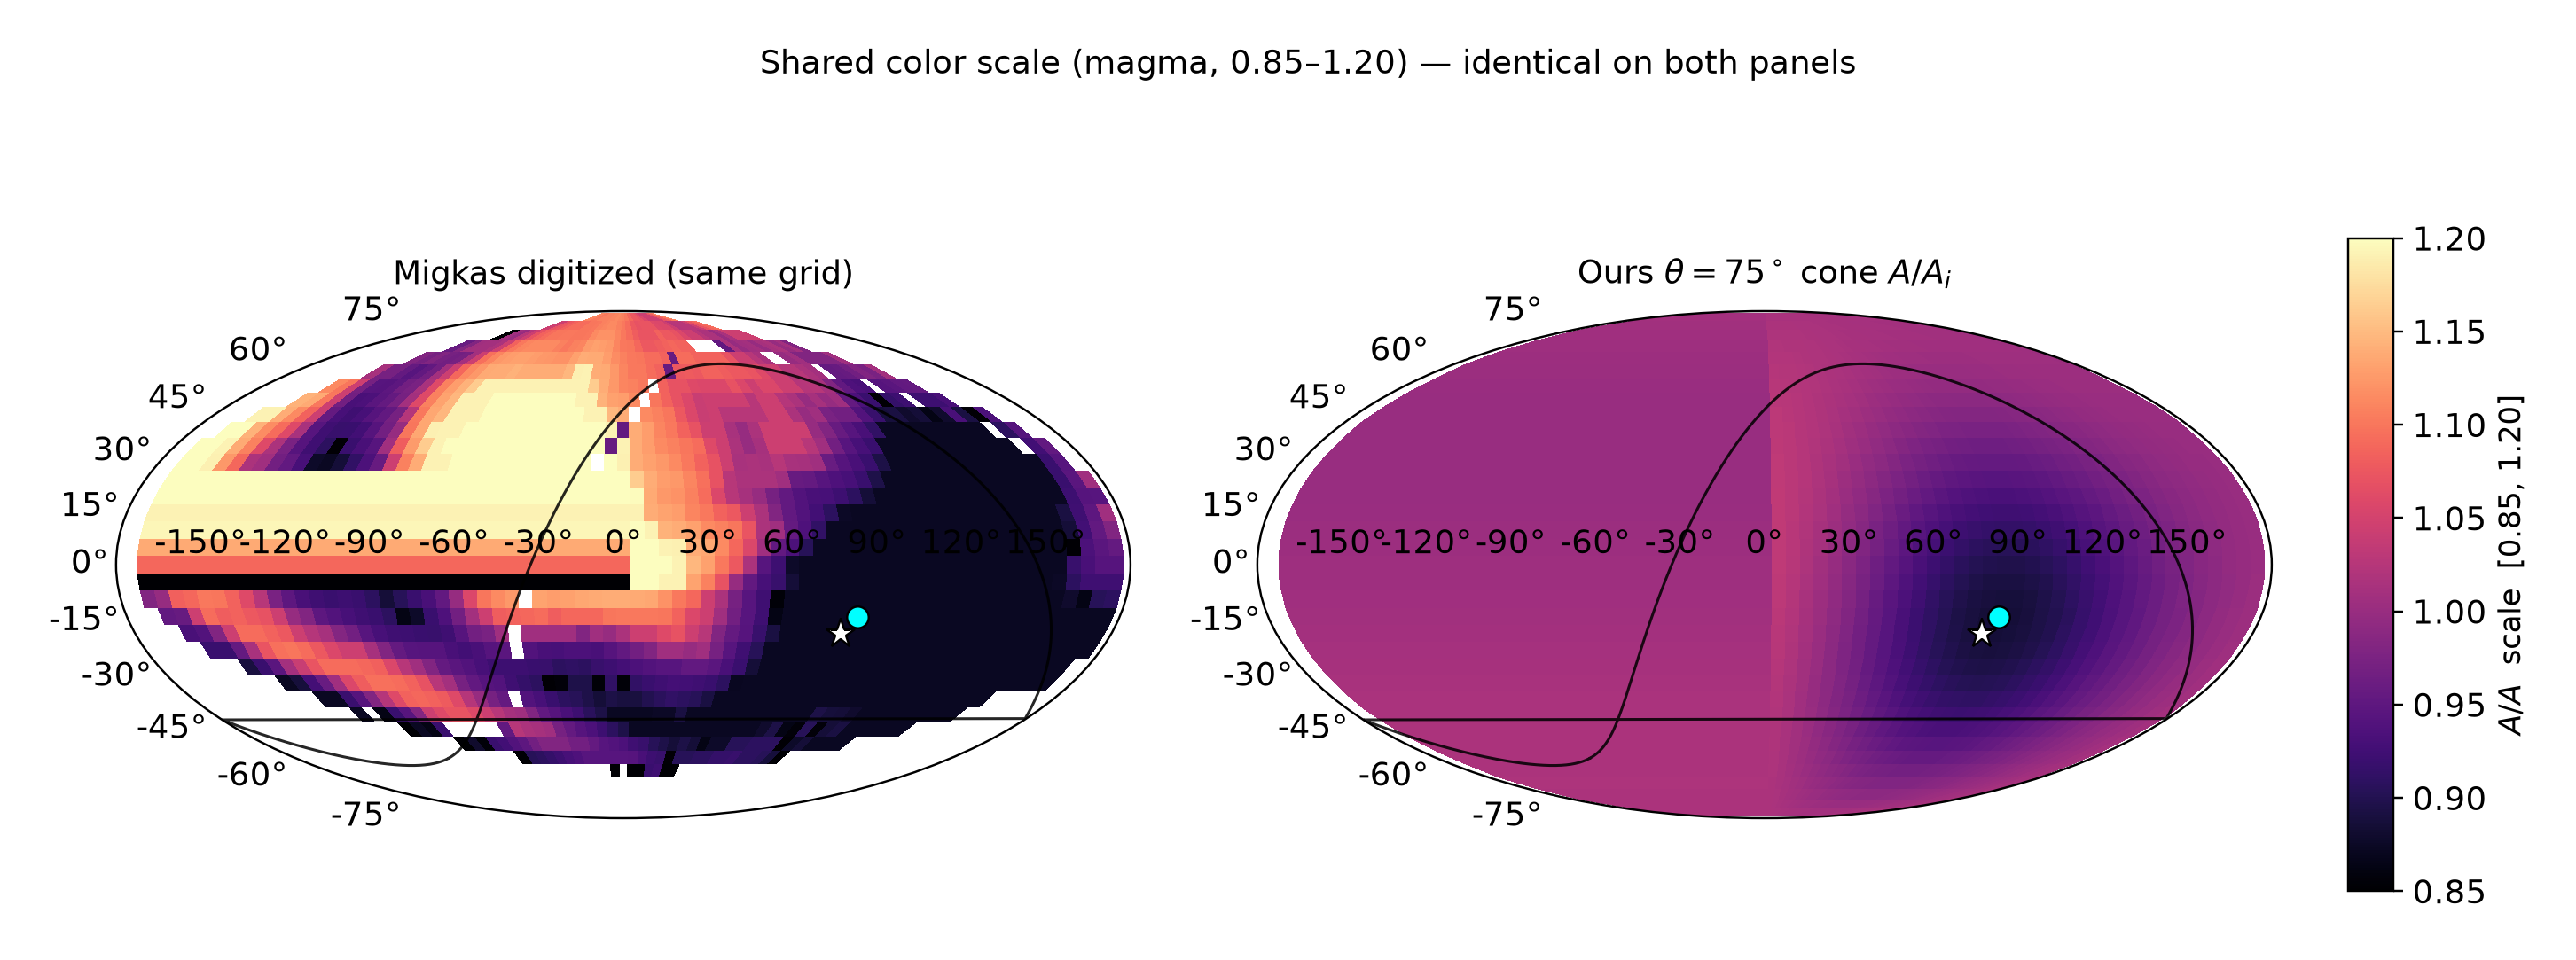
\includegraphics[width=0.88\textwidth]{sbs_SHARED_SCALE_both_mollweide.png}
\caption{Side-by-side shared-scale Mollweide comparison product from
\texttt{map\_compare/} (program archive).}
\label{fig:sbs}
\end{figure}

\begin{figure}[ht]
\centering
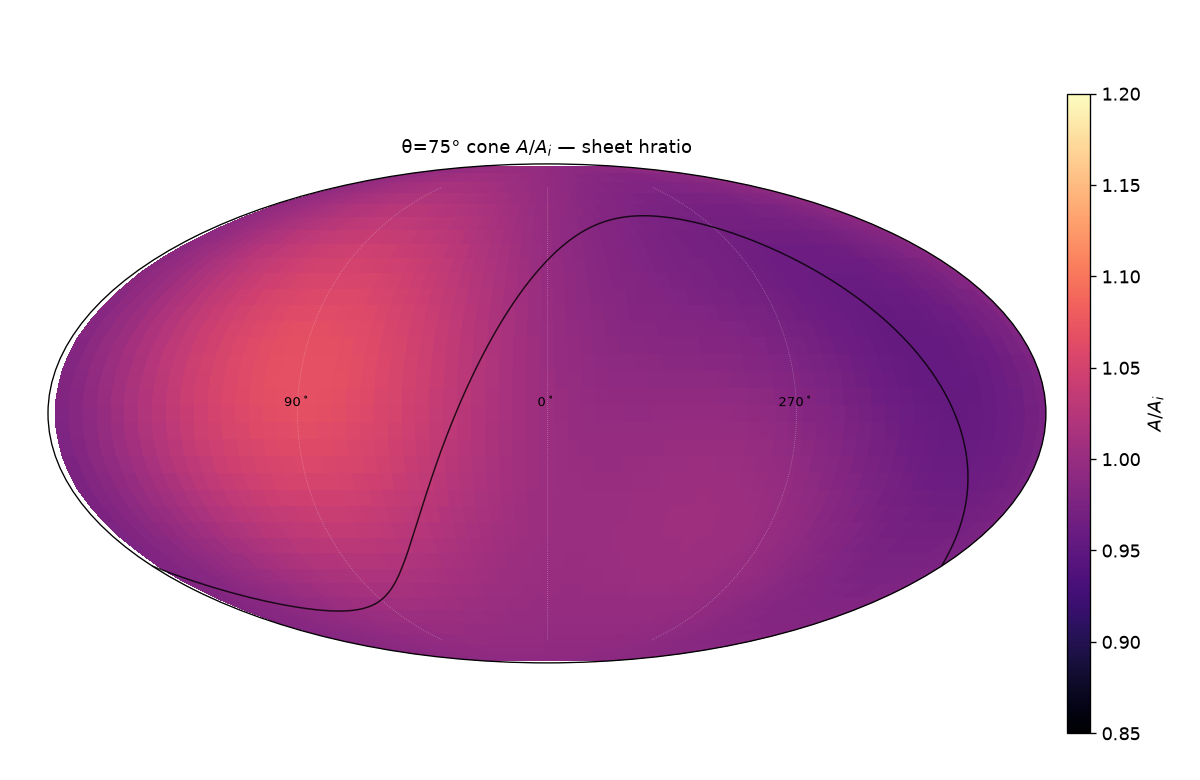
\includegraphics[width=0.72\textwidth]{CARD_theta75_sheet_hratio.png}
\caption{Example CARD sky map: $\theta=75^\circ$ cone, sheet $H$-ratio
(from \texttt{map\_compare/cone\_thetas/cards/}).}
\label{fig:card}
\end{figure}

\begin{figure}[ht]
\centering
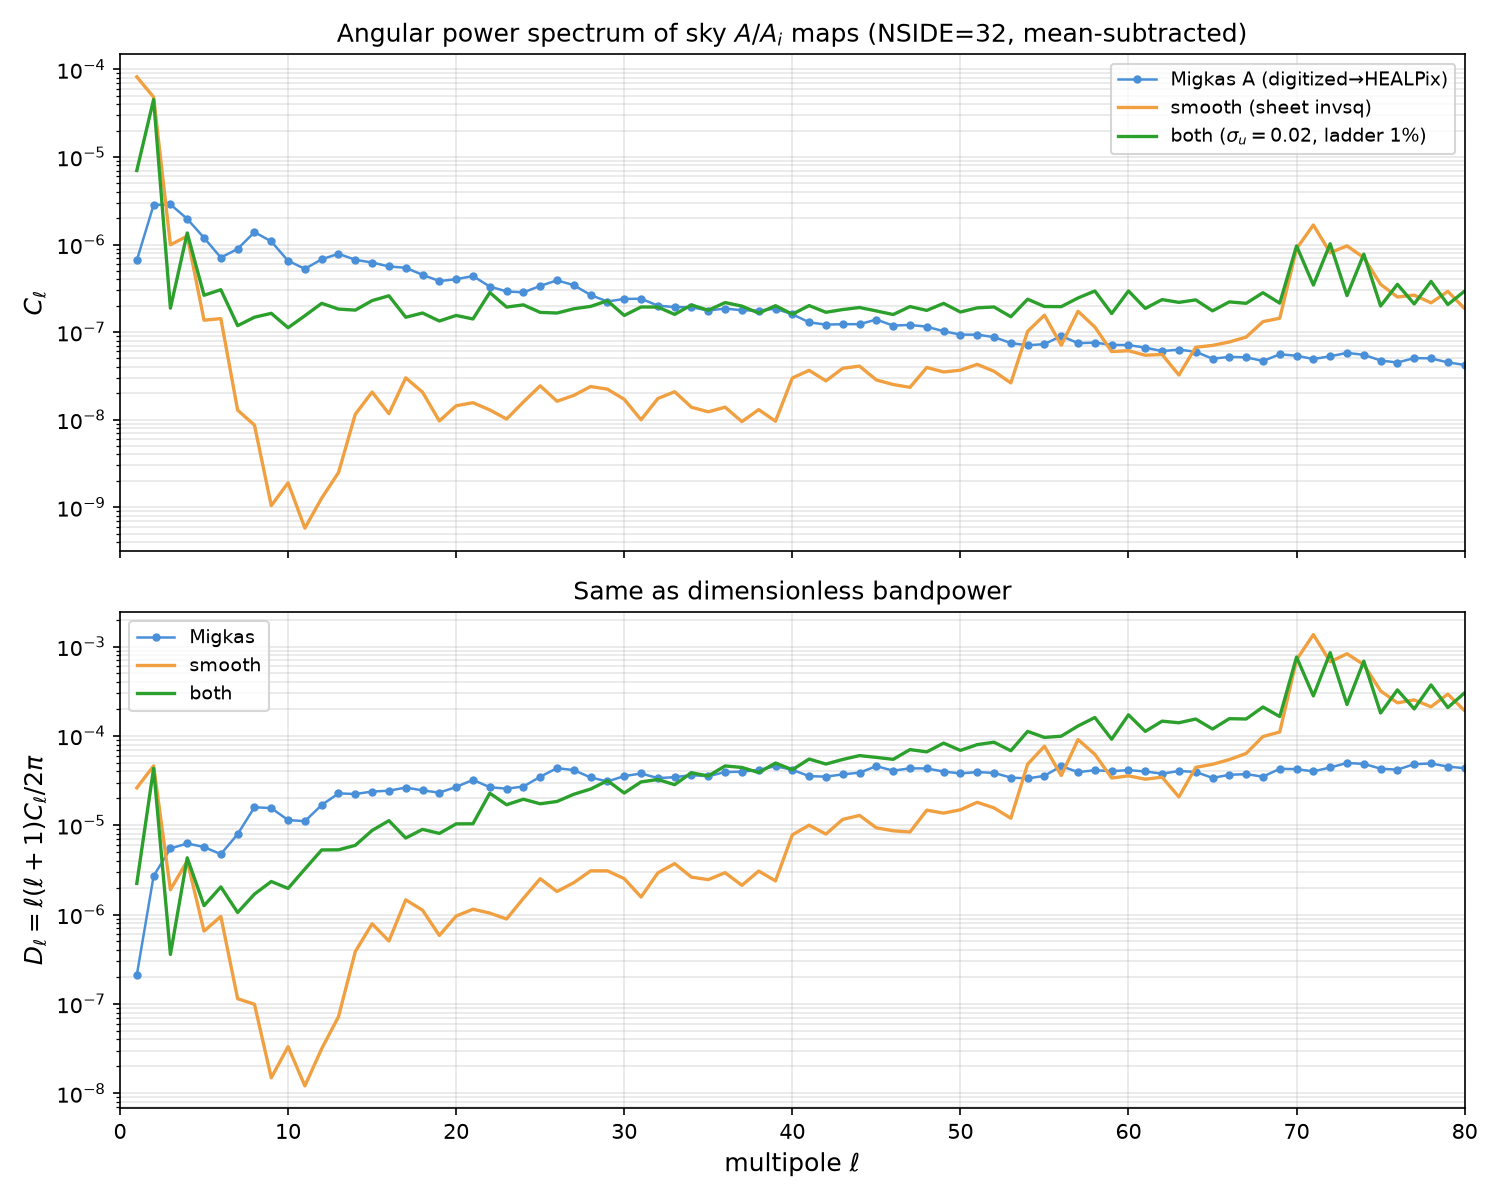
\includegraphics[width=0.78\textwidth]{Cl_A_migkas_smooth_both.png}
\caption{$C_\ell$ / smoothed $A$ map product associated with Migkas-smooth
comparisons (\texttt{Cl\_A\_migkas\_smooth\_both.png}).}
\label{fig:Cl}
\end{figure}

%======================================================================
\section{Stage setting / work remaining for a true best fit}
\label{sec:remaining}

This note stages the Newtonian ladder. It is not a finished cosmological fit.
Much work remains:

\begin{itemize}[leftmargin=*,itemsep=3pt]
\item \textbf{Joint $A{+}B$ likelihood}, not $A$-first then associated $B$.
\item \textbf{3D axis} (longitude + latitude) instead of a longitude-circle
  phase only; lock or float against Planck $|b|$ with explicit hot/cold
  convention.
\item \textbf{Time-integrated gravity} end-to-end in the likelihood (not only
  amplitude rescaling after a frozen snapshot).
\item \textbf{Selection and survey geometry} for Migkas-like cluster samples
  (mask, redshift slice, Malmquist / absorption systematics).
\item \textbf{Replace Amp$\times\sin$ and $2\ell$} with physics-derived
  quadrupole / line-of-sight depth effects, or retire them and report geometry
  alone.
\item \textbf{Ideal continuous vs discrete grid}: reconcile
  $(d/D,D/L,\kappa)$ posteriors with shared conventions for $A$ normalization.
\item \textbf{CMB}: move from flux-shell toys to last-scattering and ISW in a
  metric model; keep Alnes/Kodama-class bounds as adversaries.
\item \textbf{Honest error model}: digitize uncertainties, covariance across
  $\ell$ bins, and look-elsewhere for Amp--$\phi$--$\varepsilon$ scans.
\end{itemize}

%======================================================================
\section{Relativity required}
\label{sec:GR}

Newtonian ST+Gauss is scaffolding. A real CoE beyond the horizon, null
geodesics, and the CMB demand a relativistic inhomogeneous model---LTB or a
close cousin---as the next chapter. The existing draft
\texttt{papers/gr\_ch2\_ltb\_2026-09-20/main.pdf}
sketches that program. Priority order (Chris): get the Hubble / Migkas side
right first; park Alnes/Kodama-class CMB dipole bounds as the principal
adversary rather than pretending the Newtonian shell toy closes the case.
Until a metric model carries both $H_{\mathrm{obs}}(\hat{n})$ and the CMB,
claims of a ``best fit universe'' remain premature.

%======================================================================
\section*{Acknowledgments}
Conversations and genesis: Wolfgang Rindler; Luke Ackerman.

\begin{thebibliography}{99}

\bibitem{Migkas2020}
K.~Migkas, G.~Schellenberger, T.~H.~Reiprich, F.~Pacaud, M.~E.~Ramos-Ceja, and
L.~Lovisari,
``Probing cosmic isotropy with a new X-ray galaxy cluster sample through the
$L_X$--$T$ scaling relation,''
\textit{Astron.\ Astrophys.} \textbf{636}, A15 (2020).

\bibitem{Planck2018I}
Planck Collaboration,
``Planck 2018 results. I. Overview and the cosmological legacy of Planck,''
\textit{Astron.\ Astrophys.} \textbf{641}, A1 (2020).

\bibitem{Fixsen2009}
D.~J.~Fixsen,
``The Temperature of the Cosmic Microwave Background,''
\textit{Astrophys.\ J.} \textbf{707}, 916 (2009).

\bibitem{Alnes2006}
H.~Alnes and M.~Amarzguioui,
``CMB anisotropies seen by an off-center observer in a spherically symmetric
inhomogeneous universe,''
\textit{Phys.\ Rev.\ D} \textbf{74}, 103520 (2006).

\bibitem{Kodama2010}
H.~Kodama, K.~Saito, and A.~Ishibashi,
``Analytic solutions for the constrained cosmological perturbation equations
in the matter-dominated era and CMB anisotropies,''
related LTB / off-center CMB literature as cited in program digests (2010).

\end{thebibliography}

\end{document}
